\documentclass[10pt, conference, compsocconf]{IEEEtran}

\usepackage{times}
\usepackage{fullpage}
\usepackage{url}
\usepackage{graphicx}
\usepackage{amssymb}
\usepackage{algorithm}
% \usepackage{algpseudocode}
\usepackage[noend]{distribalgo}
\usepackage{fixme}
\usepackage{alltt}
\usepackage{xspace}
\usepackage{adjustbox}
\usepackage[usenames,dvipsnames,svgnames,table]{xcolor}
\usepackage[dvipsnames]{xcolor}
\usepackage{caption}
\usepackage{subcaption}

\newcommand{\ex}{$\mathcal{E}$}
\newcommand{\pp}{$\mathcal{P}$}
\newcommand{\ppm}{\mathcal{P}}
\newcommand{\pqm}{\mathcal{Q}}
\newcommand{\oom}{\mathcal{O}}
\newcommand{\oo}{$\mathcal{O}$}
\newcommand{\cc}{$\mathcal{C}$}
\newcommand{\ccm}{\mathcal{C}}
\newcommand{\kk}{$\mathcal{K}$}
\newcommand{\vv}{$\mathcal{V}$}
\newcommand{\vvm}{\mathcal{V}}
\newcommand{\vvt}{$\mathcal{V}$}
\newcommand{\rr}{$\mathcal{R}$}
\newcommand{\rrm}{\mathcal{R}}
\newcommand{\sst}{$\mathcal{S}$}
\newcommand{\ssm}{\mathcal{S}}
\newcommand{\ip}{\mathcal{I}}

\newcommand{\rmcast}{r-mcast}
\newcommand{\rmdel}{r-deliver}
\newcommand{\amcast}{a-mcast}
\newcommand{\amdel}{a-deliver}
\newcommand{\parts}{partition}
\newcommand{\coloralgo}{Yellow}

\newcommand{\libname}{\mbox{$libRdmaMCast$}\xspace}

\newcommand{\mynote}[3]{
   \fbox{\bfseries\sffamily\scriptsize#1}
   {\small$\blacktriangleright$\textsf{\emph{\color{#3}{#2}}}$\blacktriangleleft$}}
\newcommand{\fp}[1]{\mynote{Fernando}{#1}{Red}}
\newcommand{\lle}[1]{\mynote{Long}{#1}{Cerulean}}

\newcommand{\red}[1]{\textit{\textcolor{red}{#1}}}


\newcommand{\rwrite}{\mbox{\textsl{r-write}}\xspace}
\newcommand{\lread}{\mbox{\textsl{l-read}}\xspace}
\newcommand{\rread}{\mbox{\textsl{r-read}}\xspace}
\newcommand{\WRITE}{\textsl{WRITE}}
\newcommand{\READ}{\textsl{READ}}
\newcommand{\SEND}{\textsl{SEND}}
\newcommand{\RECV}{\textsl{RECV}}
\newcommand{\REVOKEPERM}{\textsl{REVOKE PERMISSION}}
\newcommand{\GRANTPERM}{\textsl{GRANT PERMISSION}}
\newcommand{\buffer}{\mathcal{B}}

% \newcommand{\StatexIndent}[1][3]{%
%   \setlength\@tempdima{\algorithmicindent}%
%   \Statex\hskip\dimexpr#1\@tempdima\relax}
% \algdef{S}[WHILE]{WhileNoDo}[1]{\algorithmicwhile\ #1}%


\newtheorem{lemma}{Lemma}
\newtheorem{proposition}{Proposition}
\newtheorem{theorem}{Theorem}
\newtheorem{definition}{Definition}

% do not change these values
\baselineskip 12pt
\textheight 9in
\textwidth 6.5in
\oddsidemargin 0in
\topmargin 0in
\headheight 0in
\headsep 0in

\begin{document}

\title{RamCast: RDMA-based Atomic Multicast}
% \author{Long Hoang Le, Enrique Fynn, Mojtaba Eslahi-Kelorazi, Robert Soul\'{e} and Fernando Pedone \\
% \small {\em  Universit\`{a} della Svizzera italiana (USI)} \\
% \small {\em Lugano, Switzerland} \\ [2mm]
%% \small Submission type: Research
% }
\date{}
\maketitle

% \thispagestyle{empty}
% \onecolumn
% \begin{algorithm}[h!]
\footnotesize

\begin{distribalgo}[1]

\INIT
	\STATE $ts \leftarrow 0$
	\COMMENT{P's logical clock}
	\STATE $pending \leftarrow \emptyset$
	\COMMENT{set of message to be ordered}
	\STATE $ordered \leftarrow \emptyset$
	\COMMENT{set of message already ordered, to be delivered}
	\STATE $pending_{ts} \leftarrow \emptyset$
	\COMMENT{set of pending timestamps}
	\STATE $c_\omega \leftarrow 0$
	\COMMENT{P's write counter}
	\STATE $c_r \leftarrow 0$
	\COMMENT{P's read counter}
	\STATE $\buffer \leftarrow NULL$
	\COMMENT{P's local buffer}
	\vspace{2.0mm}
\ENDINIT
\vspace{2.0mm}

\INDENT{\colorbox{\coloralgo}{to enqueue message m	:}}
	\FORALL {$p \in G \mid \forall G \in  m.dest$}
		\TRIGGER {$ \langle rdma, \WRITE \mid p, [m] \rangle$}
		\COMMENT{remote-write m to memory of all processes belong to all involved groups}
	\ENDFOR
\ENDINDENT
\vspace{2.0mm}

\INDENT{\colorbox{\coloralgo}{leader process $P_L$ of group $G$}}
	\UPON[on receive message $m$ in local buffer]{$\langle \buffer, \READ \mid m \rangle$}
		\STATE $dest \leftarrow \{\forall p \mid p \in G\} \cup \{\forall p \in G_i \mid G_i \in m.dest\}$
		\COMMENT{set of all processes in G and all leaders of involved groups}
		\STATE $ts \leftarrow ts + 1$
		\COMMENT{increase local timestamp}
		\STATE $c_\omega \leftarrow c_\omega + 1$
		\COMMENT{increase write counter}
		\FORALL {$p \in dest$}
			\TRIGGER {$ \langle rdma, \WRITE \mid p, [P_L, ts, c_\omega] \rangle$}
			\COMMENT{remote-write $P_l$'s timestamp with order $c_\omega$ to all process $\in dest$ set}
		\ENDFOR
	\ENDUPON
	\vspace{2.0mm}

	\UPON[on receive timestamp $ts_l$ of a leader $P_l$ in local buffer]{$\langle \buffer, \READ \mid [P_l, ts_l, c] \rangle$}
		\STATE $c_\omega \leftarrow c_\omega + 1$
		\COMMENT{increase write counter}
		\FORALL {$p \in G$}
			\TRIGGER {$ \langle rdma, \WRITE \mid p, [P_l, ts, c_\omega] \rangle$}
			\COMMENT{propagate $P_l$'s timestamp $ts_l$ and write counter $c_\omega$ to all process $\in dest$ set}
		\ENDFOR
		% \STATE $\forall p \in G: \rwrite(p, ts_l, c_\omega)$
		% \COMMENT{propagate $P_l$'s timestamp $ts_l$ and write counter $c$ to all process $\in dest$ set}
		\STATE $ts \leftarrow max(ts, ts_l)$
	\ENDUPON
\ENDINDENT
\vspace{2.0mm}

\INDENT{\colorbox{\coloralgo}{any process $P$ of group $G$}}
	\UPON[on receive message $m$ in local buffer]{$\langle \buffer, \READ \mid m \rangle$}
		% \STATE do $\READ(ts, L)$
		\STATE $pending \leftarrow pending \cup \{m\}$
		\COMMENT{include m in pending messages set}
		% \COMMENT{polling timestamp of leader of its own group}
	\ENDUPON
	\vspace{2.0mm}

	\UPON[on receive timestamp $ts_l$ for message $m$ in local buffer]{$\langle \buffer, \READ \mid [ts_l, c_w, m] \rangle$}
		\STATE $ts \leftarrow max(ts, ts_l)$
		\COMMENT{Lamport’s rule to update logical clocks}
		\FORALL {$p \in m.dest$}
			\TRIGGER {$ \langle rdma, \WRITE \mid p, [P, ack] \rangle$}
			\COMMENT{remote-write P's ack to memory of all involved processes}
		\ENDFOR
		% \STATE $\rwrite(p \mid p \in dest, ack)$
		\STATE $pending_{ts} \leftarrow pending_{ts} \cap \{\langle ts_l, c_w, m \rangle\}$
		\COMMENT{include $\langle ts_l, c_w, m \rangle$ in pending timestamps set}
		\vspace{1.0mm}

		\WHILE{$\exists \langle ts_l, c_w, m\rangle \in pending_{ts} : c_w = c_r + 1$}
			\STATE $pending_{ts} \leftarrow pending_{ts}$ \textbackslash $\{\langle ts_l, c_w, m\rangle\}$
			\COMMENT{remove $\langle ts_l, c_w, m \rangle$ from pending set}
			\STATE  $c_r = c_r + 1$
			\COMMENT{increase read counter}
		\ENDWHILE

		\WHILE[]{$\exists m \in pending : isFulfilled(m) = true$}
			\STATE $t \leftarrow max(ts_i)$
			\COMMENT{$t$ is the largest timestamp between all timestamps $ts_i$ populated by all leaders}
			\STATE $pending \leftarrow pending$ \textbackslash $\{m\}$
			\COMMENT{remove $m$ from pending set}
			\STATE $ordered \leftarrow ordered \cup \langle m, t \rangle$
			\COMMENT{include $\langle m, t \rangle$ in ordered set}
		\ENDWHILE

		% \WHILE {$\exists \langle m,t \rangle \in ordered : t < min(\forall t_i \in pending) \wedge \newline
		% 		\hspace*{11.7em} t < min(\forall t_i \in ordered)$:}
		\WHILE {$\exists \langle m,t \rangle \in ordered : t < min(\forall t_i \in pending) \wedge t < min(\forall t_i \in ordered)$:}
			\STATE $ordered \leftarrow ordered$ \textbackslash $\{m\}$
			\STATE deliver $m$
		\ENDWHILE
	\ENDUPON
\ENDINDENT
\vspace{4.0mm}

% \INDENT{\colorbox{\coloralgo}{\textbf{function} \rwrite$(dest, data\dots)$}}
% 	\STATE rdma-write $[data\dots]$ to $dest$'s shared buffer
% \ENDINDENT
% \vspace{2.0mm}

% \INDENT{\colorbox{\coloralgo}{\textbf{function} \READ$(data\dots)$}}
% \STATE atomic-read $[data\dots]$ from local buffer
% \ENDINDENT
% \vspace{2.0mm}

\INDENT{\colorbox{\coloralgo}{\textbf{function} isFulfilled$(m)$}}
	\IF[m receives ts of all involved groups and acks from majority processes]{$\forall G \mid G \in m.dst \wedge \newline
	\hspace*{3.5em} ts_G \neq 0 \wedge \newline
	\hspace*{3.5em} \langle ts_G, m \rangle \notin pending_{ts} \wedge \newline
	\hspace*{3.5em} $ receive acks for $ts_G$ from majority:}
		\RETURN true
	\ELSE
		\RETURN false
	\ENDIF
\ENDINDENT

\caption{RDMA Scalable Message Queue}
\label{alg:client_proxy}
\end{distribalgo}
\end{algorithm}

%!TEX root =  main.tex
\begin{abstract}
Atomic multicast is a group communication abstraction useful in the design of highly available and scalable systems.
It allows messages to be addressed to a subset of the processes in the system reliably and consistently.
All existing atomic multicast algorithm to date are based on the message-passing model.
The paper presents \libname, the first atomic multicast protocol that uses shared memory by means of Remote Direct Memory Access (RDMA).
We design \libname by leveraging RDMA technology and by carefully
combining techniques from message-passing and shared-memory systems. 
We show experimentally that \libname is significantly faster than prior systems.
\end{abstract}
%!TEX root =  main.tex
\section{Introduction}
\label{sec:introduction}

Today's online services are expected to operate uninterruptedly despite server failures.
Many such services must also be capable of handling ever-increasing demand without performance hiccups.
Services that match these expectations are deemed highly available and scalable.
Many years of intense research in the area of dependable distributed systems have deepened the understanding of how to design systems that can tolerate failures.
A golden rule in the design of such systems is that abstractions can significantly reduce complexity, and avoid design and programming errors.
For example, state machine replication, a \emph{de facto} standard to fault tolerance, requires replicas to order requests.
But ordering requests in a distributed system prone to failures is difficult \cite{FLP85}.
By relying on atomic broadcast, an abstraction equivalent to consensus \cite{HT93,CT96}, system designers can decompose ordering from execution in state machine replication, as atomic broadcast provides reliable and ordered delivery of requests.

In order to both scale performance and tolerate failures, service state is typically sharded and each shard is replicated (e.g., \cite{CDE12,Long2019,Aguilera:2007}).
Atomic multicast is a group communication abstraction that generalizes atomic broadcast by allowing requests to be propagated to groups of processes (in this case shards) with reliability and order guarantees.
Intuitively, all non-faulty processes addressed by a request must deliver the request and processes must agree on the order of delivered requests.
Atomic multicast offers strong communication guarantees and should not be confused with network-level communication primitives (e.g., IP-multicast), which offer ``best-effort" guarantees.

Since messages can be multicast to different sets of destinations and interleave in non-obvious ways, implementing message order in a distributed setting is challenging.
Some atomic multicast protocols address this challenge by ordering all messages using a fixed group of processes or involving all groups, regardless of the destination of the messages.
To be efficient, however, an atomic multicast algorithm must be \emph{genuine}: only the message sender and destination processes should communicate to propagate and order a multicast message~\cite{GS01b}.
A genuine atomic multicast is the foundation of scalable and fault-tolerant systems, since it does not depend on a fixed group of processes, and ensures reliable communication \cite{Coelho2017}.

All existing atomic multicast algorithms to date assume the message-passing system model (e.g., \cite{Coelho2017,gotsman2019white,birman1987reliable, delporte2000fault, bezerra2015ridge,
marandi2012multi}).
This paper presents \libname, the first atomic multicast protocol tailor-made for the shared-memory model.
Our motivation is practical: recent years have seen widespread development of a technology known as Remote Direct Memory Access (RDMA).
RDMA extends the traditional send and receive communication primitives with read and write operations on shared memory.
Essentially, RDMA provides a node with the capability to read and write the memory of another node, without involving the processor of this node.
In addition, RDMA offers the possibility for a process to safeguard its memory by specifying which processes can read or write which regions of its memory.
This guarantee has been shown to be quite powerful \cite{Aguilera2019}.
In particular, if every process revokes the write permission of other processes before writing to shared memory, then a process that writes successfully knows that it executed in isolation, without having to take additional steps (e.g., reading the memory). 
Protocols can leverage this property to optimize performance \cite{Aguilera2019}.

Designing an efficient RDMA-based atomic multicast protocol is not trivial, since RDMA's communication primitives vary substantially in performance.
Figure~\ref{fig:perfcomp} compares the performance of TCP/IP to RDMA's send/receive and read/write operations (setup details are presented in \S\ref{sec:evaluation:setup}).
RDMA's primitives largely outperform TCP/IP communication because they bypass the network stack.
Shared-memory RDMA primitives deliver superior performance than message-passing primitives, although the advantage depends on the message size.
In our environment, RDMA read and write operations have similar performance, unless the write can ``inline" data (i.e., with 64-byte messages in our case)---this happens because the interface adapter has the data available and does not need to retrieve data from the memory.
\libname uses remote writes only and avoids remote reads.
There are two reasons for this design.
First, most writes are small (e.g., acknowledgments) and can be inlined.
Second, a process detects a write in shared memory with busy-polling reads, and reading from a process's own memory is faster than reading from the memory of another process.
Consequently, process $p$ can read process $q$'s write more efficiently when $q$ issues a (remote) write on $p$'s memory and $p$ issues busy-polling reads on its own memory.  

\begin{figure}[htp!]
    \centering
    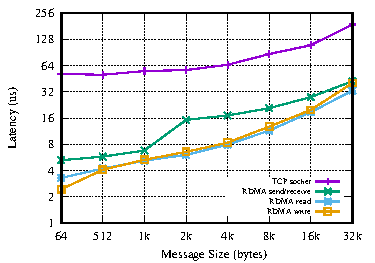
\includegraphics[width=0.99\columnwidth]{figures/benchmark/graphs/figure-protocol-bench.pdf}
  \caption{Performance comparison between communication primitives}
  \label{fig:perfcomp}
\end{figure}

In order to deliver performance that largely outperforms the most efficient message-passing atomic multicast protocols, \libname combines ideas from Skeen's genuine atomic multicast algorithm \cite{BJ87b}, a blocking algorithm that has been used as the basis for fault-tolerant atomic multicast protocols (e.g., \cite{Coelho2017,gotsman2019white}), the leader-follower replication model, explored by atomic multicast and broadcast protocols (e.g., \cite{gotsman2019white,Junqueira2011,Mu}), and Remote Direct Memory Access technology, recently used to boost the performance of distributed systems (e.g., \cite{Aguilera2019,kalia2014using, kalia2016design, mitchell2013using}).

In addition to introducing \libname, the first shared-memory genuine atomic multicast algorithm, we have implemented and evaluated \libname under various conditions. 
We show that \libname outperforms current state-of-the-art atomic multicast protocols by up to 3.7$\times$ and reduces latency by up to 20$\times$.
%MORE DATA HERE FROM THE EXPERIMENTAL EVALUATION

The remainder of the paper is structured as follows.
Section~\ref{sec:background} presents the system model, a formal definition of the atomic multicast problem, and the basics of Remote Direct Memory Access.
Section~\ref{sec:rdma-atomic-multicast} details the \libname protocol.
We start with a short description of the ideas that have inspired \libname, then describe its normal behavior, in the absence of failures, and how it handles failures.
Section~\ref{sec:implementation} describes our prototype, and Section~\ref{sec:experimental-evaluation} presents the performance evaluation.
Section~\ref{sec:related-work} surveys related work and Section~\ref{sec:conclusion} concludes the paper.


%!TEX root =  main.tex

\clearpage
\section{Background}
\label{sec:background}

In this section, we present the system model (\S\ref{sec:system-model}), define the atomic multicast communication problem (\S\ref{sec:amcast}), and quickly overview RDMA, the key enabling technology used in this work (\S\ref{sec:rdma}).

\subsection{System model}
\label{sec:system-model}

We assume a hybrid distributed system model in which processes can use both message-passing and shared-memory \cite{Aguilera2019}.
The system is composed of a set of client and server processes, which communicate by exchanging messages or accessing portions of each other's memory.
Processes are \emph{correct}, if they do not fail, or \emph{faulty}, otherwise. 
In either case, processes do not experience arbitrary behavior (i.e., no Byzantine failures).
Our protocols ensure safety under both asynchronous and synchronous execution periods. 
To ensure liveness, we assume the system is \emph{partially synchronous} \cite{DLS88}, 
that is, it is initially asynchronous and eventually becomes synchronous. The time when the 
system becomes synchronous is called the \emph{Global Stabilization Time (GST)}, and it is unknown to the processes.
Before GST, there are no bounds on communication and processing delays; after GST, such bounds exist but are unknown. 

A process can share memory regions with other processes and define permissions for those shared memory regions. 
Process $q$ can read and write a register $v$ in $p$'s memory region $mr$ with operations $\textsf{read}(p,v)$ and $\textsf{write}(p,v,value)$, respectively.
A permission associated with memory region $mr$ defines disjoint sets of processes $R_{mr}, W_{mr}, RW_{mr}$ that can read, write, or read-write the registers in region $mr$. 
Process $q$ has permission to read (respectively, write and read-write) $v$ in $p$'s $mr$ if $q \in R_{mr}$ (resp. $W_{mr}, RW_{mr}$).
A process can initially assign permissions for its shared memory regions and later change these permissions.

Processes can also communicate by exchanging messages over a set of directed links using primitives \textsf{send}$(p, m)$ and \textsf{receive}$(m)$, where $p$ is the addressee of message $m$.
We assume messages are unique.
Communication links are reliable in that every message sent by a process $p$ to another process $q$ is guaranteed to be eventually delivered by $q$ if both $p$ and $q$ are correct.
Moreover, a message is received at most once, and only if it was previously sent.


\subsection{Problem statement}
\label{sec:amcast}

Let $\Pi = \{p_1, p_2, ...\}$ be the set of server processes.
We define $\Gamma \in 2^{\Pi}$ as the set of process groups in the system. 
Groups are disjoint and each group contains $2f+1$ processes, where $f$ is the maximum number of faulty processes per group.  
The assumption of disjoint groups has little practical implication since it does not prevent collocating processes that are members of different groups on the same machine.
A set of $f + 1$ processes in group $g$ is a \emph{quorum} in $g$.

A process atomically multicasts a message $m$ to groups in $m.dst$ by invoking primitive multicast($m$), where $m.dst$ is a special field in $m$ with $m$'s destinations; a process delivers $m$ with primitive deliver($m$). 
We define the relation $<$ on the set of messages processes deliver as follows: $m < m'$ iff there exists a process that delivers $m$ before $m'$. 

Atomic multicast ensures the following properties: 
\begin{itemize}
\item \textit{validity}:~if a correct process $p$ multicasts a message $m$, then eventually all correct processes $q \in g$, where $g \in m.\mathit{dst}$, r-deliver $m$.
\item \textit{integrity}:~for any process $p$ and any message $m$, $p$ r-delivers $m$ at most once, and only if $p \in g$, $g \in m.\mathit{dst}$, and $m$ was previously r-multicast.
\item \textit{uniform agreement}:~if a process $p$ a-delivers a message $m$, then eventually all correct processes $q\in m.\mathit{dst}$ a-deliver $m$.
\item \textit{uniform prefix order}:~for any two messages $m$ and $m'$ and any two processes $p$ and $q$ such that $p \in g$, $q \in h$ and $\{ g, h \} \subseteq m.\mathit{dst} \cap m'.\mathit{dst}$, if $p$ a-delivers $m$ and $q$ a-delivers $m'$, then either $p$ a-delivers $m'$ before $m$ or $q$ a-delivers $m$ before $m'$.
\item \textit{uniform acyclic order}:~the relation $<$ is acyclic.
\end{itemize}
Atomic broadcast is a special case of atomic multicast in which every message is addressed to all groups.

We require atomic multicast protocols to be \emph{genuine}~\cite{GS01b}: 
an algorithm ${\cal A}$ solving reliable or atomic multicast is genuine
if and only if for any admissible run $R$ of ${\cal A}$ and for any process $p$ in $R$, if $p$ sends or receives a message, then some message $m$ is multicast, and either (a)~$p$ is the process that multicasts $m$ or (b)~$p \in g$ and $g \in m.dst$.


\subsection{Remote Direct Memory Access}
\label{sec:rdma}

Remote Direct Memory Access (RDMA) is a hardware-based protocol that enables direct data access between the memory of remote machines without the involvement of the Operating System (OS) and processor. 
RDMA implements dedicated network stack implemented in its hardware, provides both low-latency and high-bandwidth by bypassing the OS kernel supports zero-copy net-working.
RDMA provides two-sided operations (e.g., send, receive), one-sided operations (e.g., read, write), and atomic operations (e.g., compare-and-swap, fetch-and-increment). The two-sided operations still have CPU involvement to remote host and user-space memory copies, thus introduces an unavoidable overhead compared to one-sided RDMA verbs \cite{FaRM}.
Beside, previous studies have established that remote write operations provide superior performance than remote reads, and send and receive operations, and much better performance than atomic operations \cite{kalia2014using, kalia2016design, mitchell2013using}.
In RamCast's normal operation, processes communicate using remote write operations only.
We refrain from using remote read operations, and resort to send and receive operations when handling failures, since they lead to simpler logic.

RDMA provides three transport modes: Reliable Connection (RC), Unreliable Connection (UC) and Unreliable Datagram (UD). 
While RC and UC are connection oriented and support only one-to-one data transmission, UD supports both one-to-one and one-to-many without establishing connections.
RC ensures data transmission is reliable and correct in the network layer, while UC doesn’t have such guarantee.
In this work, we use RC to provide in-order reliable delivery.
To establish a connection between two remote hosts, the RDMA-enabled network card (RNIC) on each host creates a logical RDMA endpoint known as a Queue Pair (QP), including a send queue and a receive queue for storing data transfer requests. 
Operations are posted to QPs as Work Requests (WRs) to be consumed and executed by the RNIC. 
When an RDMA operation is completed, a completion event is pushed to a Completion Queue (CQ).
Each host makes local memory regions (MR) available for remote access by asking its OS to pin the memory pages that would used by the RNIC.
Both QPs and MRs can have different access modes (e.g., read-only or read-write). 
The hosts specify the access mode when initializing the QP or registering the MR, but the access mode can be dynamically update later. 
The host can register the same memory for different MRs. Each MR then has its own access mode.
In this way, different remote machines can have different access rights to the same memory. 
% The same effect can be obtained by using different access flags for the QPs used to communicate with remote machines.
%!TEX root =  main.tex

\section{RamCast: RDMA-based Atomic Multicast}
\label{sec:rdma-atomic-multicast}

In this section, we recall the building blocks that inspired \libname (\S\ref{sec:bblocks}) and present its design and algorithms. 
We start with an overview of \libname (\S\ref{sec:overview}), then detail its data structures (\S\ref{sec:ds-structs}) and algorithms in the absence of failures (\S\ref{sec:normalcase}) and in the presence of failures (\S\ref{sec:failurecase}).
We conclude with a few extensions to the protocol (\S\ref{sec:extensions}).
We argue for the correctness of \libname in the Appendix.\footnote{https://www.dropbox.com/s/nlwzujxrtz5eopj/ramcast-proof.pdf?dl=0}

\subsection{Building blocks}
\label{sec:bblocks}

\libname leverages two ideas, Skeen's atomic multicast algorithm \cite{BJ87b} and Protected Memory Paxos \cite{Aguilera2019}.
Skeen's algorithm orders messages multicast to multiple processes consistently but it does not tolerate failures.
Protected Memory Paxos takes advantage of RDMA permissions to improve the efficiency of Paxos \cite{L98}. 
Like Paxos, it implements atomic broadcast (i.e., it assumes a single group of processes).
%Combining these ideas coherently and efficiently is not trivial, as we discuss in this section,
%after briefly presenting Skeen's algorithm and Protected Memory Paxos.

%\subsubsection{Skeen's atomic multicast}

\subsubsection{Skeen's atomic multicast}

In Skeen's algorithm, each process assigns unique timestamps to multicast messages based on a logical clock~\cite{Lam78}.
The correctness of the algorithm stems from two basic properties:
(i)~processes in the destination of a multicast message first assign tentative timestamps to the message and eventually agree on the message's final timestamp; and
(ii)~processes deliver messages according to their final timestamp.
These properties are implemented as follows.

\begin{itemize}
\item[(i)] To multicast a message $m$ to a set of processes, $p$ sends $m$ to the destinations.
Upon receiving $m$, each destination updates its logical clock, assigns a tentative timestamp to $m$, stores $m$ and its timestamp in a buffer, and sends $m$'s timestamp to all destinations.
Upon receiving timestamps from all destinations in $m.dst$, a process computes $m$'s final timestamp as the maximum among all received tentative timestamps for $m$.
\item[(ii)]Messages are delivered respecting the order of their final timestamp.
A process $p$ delivers $m$ when it can ascertain that $m$'s final timestamp is smaller than the final timestamp of any messages $p$ will deliver after $m$ (intuitively, this holds because logical clocks are monotonically increasing).
\end{itemize}

\subsubsection{Protected Memory Paxos}
\label{sec:PMP}

In Paxos \cite{L98}, to order a message $m$, the leader proposes $m$ in a consensus instance.
In the normal case, where there is a single leader, the followers accept the proposed message and reply to the leader.
In Protected Memory Paxos, the followers grant exclusive write permission to their memory to the leader.
If a new leader takes over, then it revokes the permission of the previous leader.
To order $m$, the leader writes $m$ in the memory of the followers.
If the leader succeeds in writing the message in the memory of a quorum of followers, then no other leader took over, and the message is ordered.

Just like Paxos, to ensure that the new leader makes decisions that are consistent with the decisions of the previous leader, each leader associates a \emph{round} to its proposed message.
%A round is a tuple $\langle rnd, pid \rangle$, where $rnd$ is a scalar and $pid$ is the process unique identifier, used to make rounds unique across the system.
Rounds are unique across the system.
%The very first leader, say process $p$, uses round $\langle 0, p \rangle$.
When process $q$ becomes leader, upon suspecting the failure of the current leader $p$, $q$ must pick a round bigger than $p$'s round.
Process $q$ then proceeds in two steps.
First, $q$ needs to acquire permission from a quorum of processes, which it does by contacting all processes and providing its chosen round.
Processes grant write permission to $q$ if the provided round is bigger than the round of the process that currently holds the write permission.
Second, $q$ must check whether other processes have already accepted any values.
If so, $q$ must propose the value that has been accepted in the largest round; otherwise, $q$ can propose a new value.

\subsection{\libname design and architecture}
\label{sec:overview}

Figure~\ref{fig:arch} depicts the various components and memory layout of \libname.
Processes within each group coordinate using the leader-follower model \cite{gotsman2019white,Junqueira2011,Mu,delta4}.
Each server process has a fixed-size buffer per client, analogously to other RDMA-based systems \cite{FaRM, Mu, DARE, APUS}.
A buffer in \libname is divided into two parts, a message buffer $M$, and a timestamp buffer $T$.
Message buffer $M$ is a shared memory region that can be read and written by any processes, including the client process the buffer is associated with.
Timestamp buffer $T$ is protected and can only be written by the leader of each group; the buffer can be read by any processes.
Each slot in $M$, with a multicast message $m$, has a corresponding slot in $T$, with $m$'s timestamp.

%Each server process organizes its memory in regions: a shared
%memory region and a protected memory region. All processes have remote access
%(read/write) to the shared memory space. 
%Only one leader of each group
%has remote-write permission to a given node's log at any point in time
%during the protocol.

Clients keep a copy of the remote head and tail pointer of their buffer at each server. 
A client increases the remote tail after writing to the shared memory. 
The server process updates the head pointer on the client buffer after handling the message.
% by piggybacking the new value in the response.
Each process $p$ periodically polls the memory cell at the head position of each
connected QPs to detect new messages.
%\libname maintain quorums of ``candidate'' processes of each group to be the leader of that group.




\begin{figure}[ht!]
  \centering
  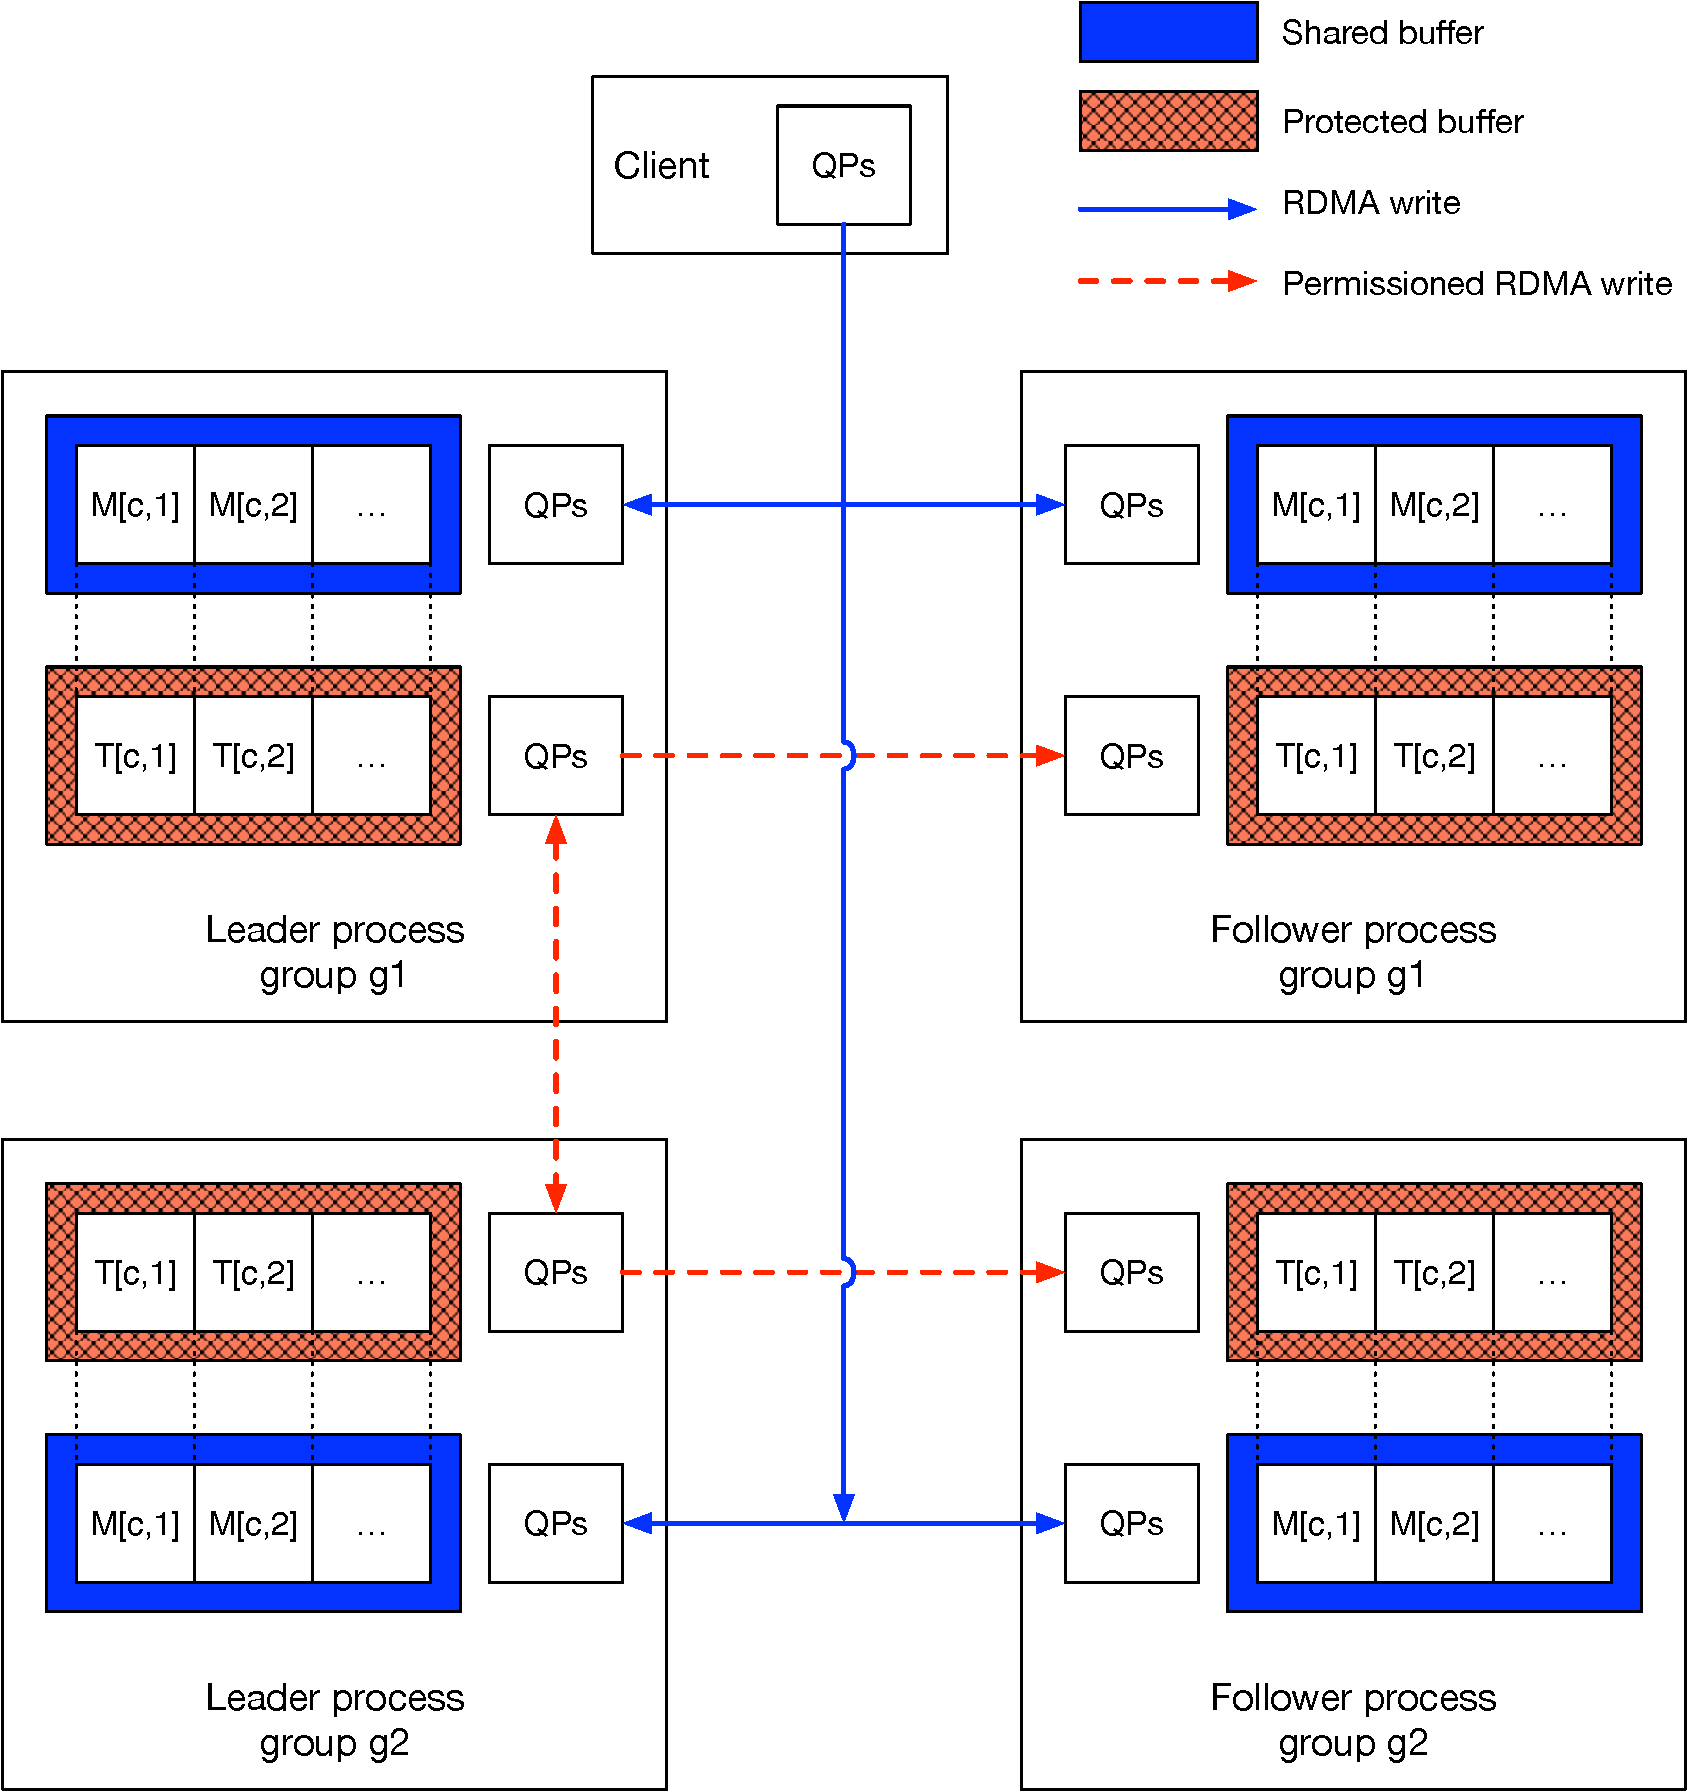
\includegraphics[width=1\linewidth]{figures/architecture2}
  \caption{\libname's memory layout. The normal execution proceeds in three steps: in step 1, the client writes a multicast message in the memory of all destination processes; in step 2 the leader of each destination group proposes and writes a timestamp for the message in the memory of its followers and other leaders; in step 3 the leaders propagate the timestamp written by other leaders, and the followers acknowledge the proposed timestamps. The message is delivered after step 3.}
%Processes have shared and exclusive memory that can be accessed by RDMA primitives. Exclusive memory access needs permission. A client proposes new message by writing to the shared memory of all processes. Leader processes writes their proposed timestamps to exclusive memory. Follower processes write their acknowledgement to the shared memory}
  \label{fig:arch}
\end{figure}


\libname consists of the following main components:
\begin{itemize}
  \item \emph{Memory management.} This component handles the shared buffer and the protected buffer (detailed in \S\ref{sec:ds-structs}). While all processes have read and write access to the shared buffer of a process, only the leader of each group has write permission to the protected buffer of a process. 
  %Each process grants and revokes write permission to its protected buffer, to ensure only one leader of each group has write access at a time.
  \item \emph{RDMA communication.} This component provides functions to read and write remote memory, used by the normal execution component, and to send and receive messages, used by the failure handling module.
  \item \emph{Normal execution.} The normal protocol execution (detailed in \S\ref{sec:normalcase}) is invoked when there is a sole leader per group with support of at least a majority of processes in its group. A leader is responsible for proposing the group's timestamp for a new multicast message, and propagating timestamps from other groups to followers of its own group.
  \item \emph{Failure handling.} Upon detecting the failure of a leader, processes in a group elect a new leader. The new leader must ensure that its execution is consistent with the execution of the previous leader (detailed in \S\ref{sec:failurecase}).
  \item \emph{Leader election.} \libname requires processes to detect a slow or crashed leader, and elect a new leader. Leader election is not assumed to be perfect: the protocol ensures safety despite multiple leaders in a group. To ensure progress, though, eventually every group should elect a single operational and stable leader \cite{Aguilera2019,L98}.
Stable leader election can be implemented in the partially synchronous model \cite{Aguilera2001}.
\end{itemize}

\subsection{Data structures}
\label{sec:ds-structs}

Algorithm~\ref{alg:data_struct} presents the data structures used by processes in \libname.
Every server process has a shared buffer $M$ per client $c$, where slot $M[c,i]$ contains the $i$-th message $msg$ multicast by client $c$, the groups $dst$ the message is addressed to, and an address vector $ptr$, where $ptr[g,p]=j$ means that at process $p$ in group $g$ message $msg$ is stored in slot $M[c,j]$. 
The address vector is used by a process to know where to write in the memory of another process addressed by the message.
Servers compute the message's timestamp $tmp$, based on the timestamps proposed by the leader of each destination group, and the acknowledgements from the members of the leader's group, stored in vector $ack$.
%A timestamp is a tuple $(cnt,pid)$, where $cnt$ is a scalar and $pid$ is a process identifier, used to break ties.
A multicast message state $stat$ can be null ($\perp$), pending a final timestamp (\mcast), assigned a final timestamp (\ordered) or delivered (\done).

To compute a message's timestamp, each server process has a protected buffer $T$, where the $i$-th slot $T[c,i]$ matches the corresponding slot $M[c,i]$ in the shared buffer $M$ associated with $c$.
The slot contains a timestamp vector $tmp$ and a round vector $rnd$, each one with an entry per group $g$: $tmp[g]$ contains the timestamp proposed by the current leader in $g$ in round $rnd[g]$.
Timestamps and rounds are tuples $\langle cnt,pid \rangle$, where $cnt$ is a scalar and $pid$ is a process identifier. 
It follows that $\langle cnt,pid \rangle > \langle cnt',pid' \rangle$ iff $cnt > cnt'$, or $cnt = cnt'$ and $pid > pid'$.
We further assume that $time(\langle cnt,pid \rangle)=cnt$.

To multicast a message, a client writes the message in the shared buffer of each process in the groups addressed by the message.
To know in which entry the multicast message must be written, the client keeps an address vector $ptr$ with an entry per group and per process in the group.

Process $p$'s local state includes a $clock$, used to compute logical timestamps, $p$'s current round, used when $p$ is the leader of the group, vector $Leader$ with $p$'s view on the current leader of each group, and vector $Round$, where entry $Round[g]$ contains the largest round $p$ has accepted from $Leader[g]$.


\begin{algorithm}
\footnotesize

\begin{distribalgo}[1]

\STATE{Each server has a shared buffer $M$ and a protected buffer $T$ per client $c$;
each slot in $M$ stores a multicast message; the corresponding slot in $T$ stores the message's timestamps}	
\vspace{1.0mm}
\INDENT{Each slot $M[c,i]$ contains the following information:}
	\STATE $msg$: the message $m$ multicast by client $c$
	\STATE $dst$: destination groups $m$ is addressed to
	\STATE $ptr[1..k,1..n]$: for each $g$ in destination, slot with $msg$ at processes in $g$; $null$ if $g$ is not in the message's destination
	\STATE $tmp$: the timestamp of $m$, initially $\langle 0,0 \rangle$
	\STATE $ack[1..k,1..n]$: for each $g$ in destination, acknowledgment of timestamp in $T[c,i].tmp[g]$ from processes in $g$
	\STATE $stat$: state of $m$: $\perp$ (initially), \mcast, \ordered\ or \done
\ENDINDENT
\vspace{1.0mm}
\INDENT{Each entry $T[c,i]$ contains the following information:}
	\STATE $tmp[1..k]$: timestamp proposed by leader of group $g$
	\STATE $rnd[1..k]$: the round of $g$'s leader, initially $\langle 0,0 \rangle$
\ENDINDENT
\vspace{1.0mm}
\STATE{Each client $c$ has vector $ptr[1..k,1..n]$, with the next available slot in buffers $M$ and $T$ per group $g$ and process $p$}
\vspace{1.0mm}

\INDENT{Each server $p$ at group $g$ also has:}
	\STATE $clock$: logical timestamp counter at $p$, initially $\langle 0,p \rangle$
	\STATE $round$: the round of $p$, when leader, initially $\langle 0,p \rangle$
	\STATE $Leader[1..k]$: the leader at each group
	\STATE $Round[1..k]$: last accepted round at each group
\ENDINDENT

\vspace{2.0mm}

%\INDENT{\textbf{procedure} $Relay(c,msg,dst,ptr)$}
%	\INDENT{for each $h$ in $dst$: for each $q$ in $h$}
%		\STATE \rdwrite{q}{M[c,ptr[q]].msg}{msg}
%		\STATE \rdwrite{q}{M[c,ptr[q]].dst}{dst}
%		\STATE \rdwrite{q}{M[c,ptr[q]].ptr}{ptr}
%		\STATE \rdwrite{q}{M[c,ptr[q]].stat}{\mcast}
%	\ENDINDENT
%\ENDINDENT
%\vspace{2.0mm}
%\INDENT{\textbf{function} $increment((cnt,pid))$}
%	\STATE $cnt \leftarrow cnt + 1$
%	\STATE return $(cnt,pid)$
%\ENDINDENT
%\vspace{2.0mm}
%
%\vspace{2.0mm}
%\INDENT{\textbf{function} $max((cnt_1,pid_1),(cnt_2,pid_2))$}
%	\IF{$cnt_1 > cnt_2$ \textbf{or} $(cnt_1=cnt_2\ \band\ pid_1 > pid_2)$}
%		\STATE return $(cnt_1,pid_1)$
%	\ELSE
%		\STATE return $(cnt_2,pid_2)$
%	\ENDIF
%\ENDINDENT
%\vspace{2.0mm}


\caption{Data structures}
\label{alg:data_struct}
\end{distribalgo}
\end{algorithm}




%\begin{figure}[ht!]
%  \centering
%  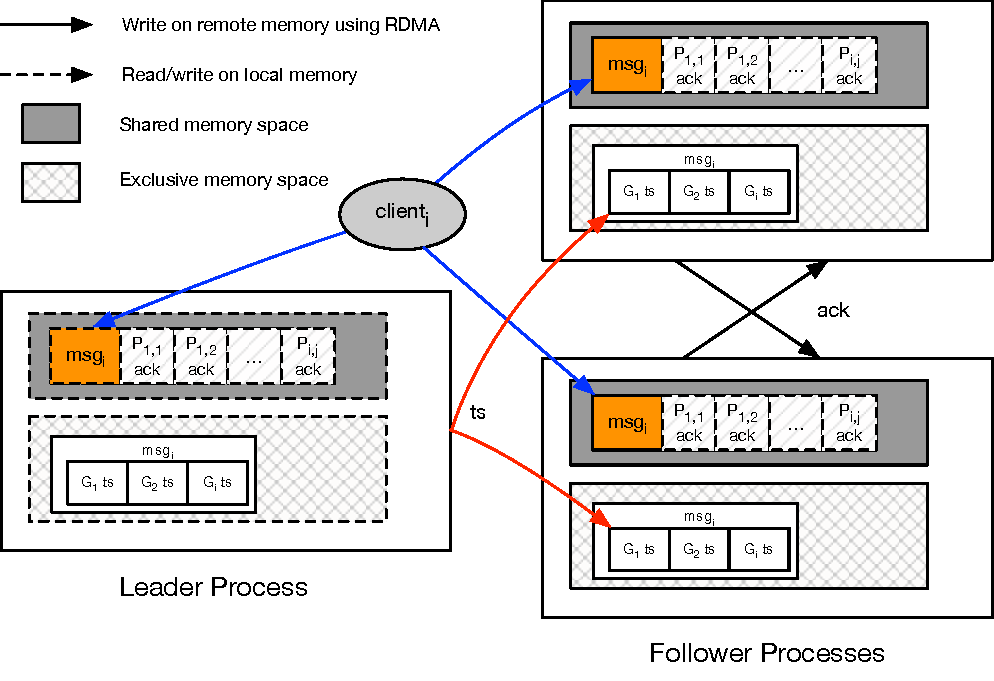
\includegraphics[width=1\linewidth]{figures/memory}
%  \caption{Memory layout of \libname. Each process has shared and exclusive memory
%  space. All other processes can access shared memory. Only leader can access
%  exclusive memory }
%  \label{fig:normal_operation_time}
%\end{figure}







\subsection{Normal execution}
\label{sec:normalcase}

\libname is optimized for the normal case, when a message is addressed to groups whose leaders are operational and stable.
Algorithm \ref{alg:normal_case} presents \libname's normal execution, and 
Figure~\ref{fig:normal_operation_time} illustrates one normal execution.
We explain next the behavior of each one of the tasks in Algorithm \ref{alg:normal_case}.

\begin{itemize}
\item \emph{Task 1.} To multicast message $m$, client $c$ first calculates the next available slot in the buffer of every process addressed by $m$. Then, $c$ invokes the $Relay$ procedure, which copies the message, its destination, and the address vector for $m$ in the message buffer of every process addressed by $m$.

\begin{figure}[ht!]
  \centering
  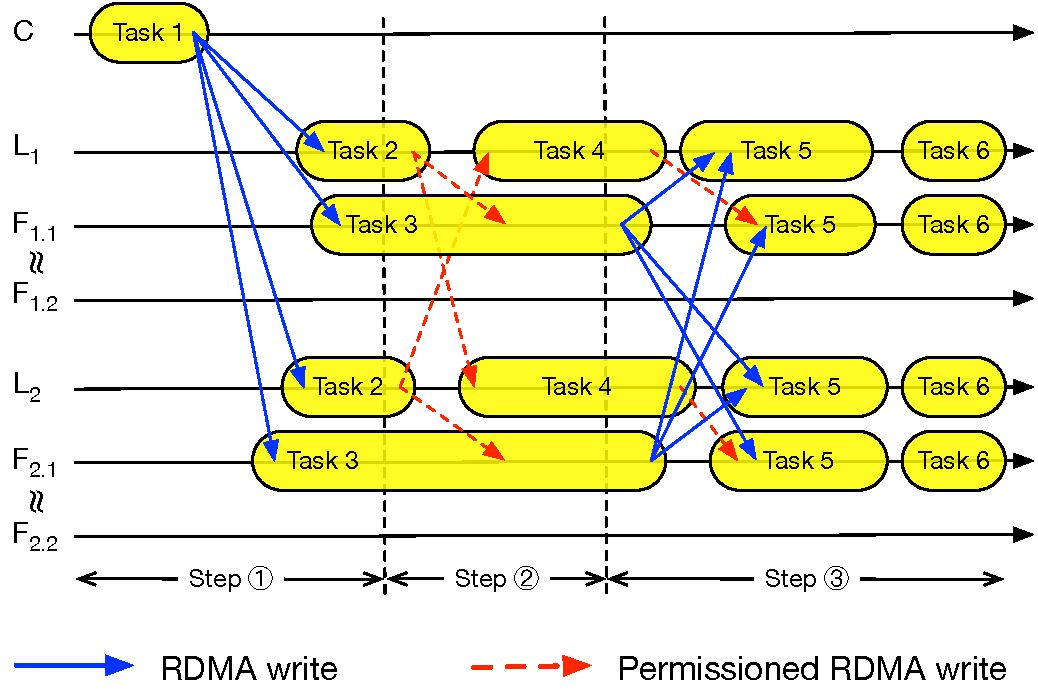
\includegraphics[width=1\linewidth]{figures/execution}
  \caption{Normal execution of \libname. We show the steps at one follower per group only to avoid cluttering.}
  \label{fig:normal_operation_time}
\end{figure}

\item \emph{Task 2.} Once leader process $L$ in group $g$ reads $m$ from its message buffer, it computes a
group-wise timestamp for $m$ and writes the proposed timestamp 
in the protected timestamp buffer of all follower processes in the leader's group $g$, and all leader processes 
of other groups in the destination of $m$.
If a remote write is denied, then $L$ ends the task since another process in $g$ became leader.

\item \emph{Task 3.} When a follower detects that a multicast message has been assigned a timestamp by the group leader, it updates its clock.
This is done to ensure that timestamps from a group are monotonically increasing (necessary in case the process becomes leader).
Then, the follower acknowledges that it has read this timestamp by writing the round used by the leader in its entry in the $ack$ vector of every process in the destination of the message.
The follower detects the leader proposed timestamp by checking whether the round of the timestamp matches the round associated with the  leader. 
This assumes that both the timestamp and the round have been updated by the leader.
We discuss in Section~\ref{sec:implementation} how we ensure this with RDMA.

\item \emph{Task 4.} 
When the leader $L$ in $g$ reads a timestamp written by a leader in another group, $L$ updates its local clock with the timestamp, to ensure that any future proposed timestmaps will be bigger, and writes the read timestamp in the memory of each one of its followers.
This task is executed by the leader of a group only, since only the leader is updated with timestamps from the leader of another group (see Task 2).
The reason why only the leader of a group is updated is to ensure that any timestamps assigned by the leader are consistent with any other timestamps assigned by the group.
%, similarly to other leader-follower-based protocols \cite{gotsman2019white, Junqueira2011}.
%Once each involved process $P$ belongs to $m.dst$ \lread message $m$ in its
%local buffer, $P$ mark the message as pending, and starts polling from it
%exclusive memory for timestamps of $m$ (Task 4 algorithm~\ref{alg:normal_case}).

\item \emph{Task 5.} 
When a message has a timestamp proposed by a leader from each destination group of the message, and a quorum of processes in each destination group agrees with the proposed timestamp, the message becomes ordered.

\item \emph{Task 6.} 
A process delivers an ordered message when it can assert that no other messages can be assigned a smaller timestamp.

\end{itemize}

In the normal case, a message multicast by a client to multiple groups is delivered by the leaders and the followers of the addressed groups after three RDMA write delays (see Figure~\ref{fig:normal_operation_time}).
In Section~\ref{sec:extensions}, we discuss how messages addressed to a single group can be delivered by the group's leader after two RDMA write delays.

%!TEX root =  main.tex

\newcommand{\rdwrite}[3]{WRITE\ensuremath{(@#1\!\rightarrow\!#2, #3)}}	% rdwrite(addr,val) 
%\newcommand{\rmm}[2]{\ensuremath{@#1\!\rightarrow\!#2}}
\newcommand{\band}{\textbf{and}}
\newcommand{\mcast}{\textsf{mcast}}
\newcommand{\ack}{\textsf{ack}}
\newcommand{\ordered}{\textsf{ordered}}
\newcommand{\done}{\textsf{done}}
\newcommand{\myack}{\textsf{ack}}

\begin{algorithm}
\footnotesize

\begin{distribalgo}[1]

\STATE{Each server has a shared buffer $M$ with multicast messages and a protected buffer $T$ with message timestamps per client $c$}	
\vspace{1.0mm}
\INDENT{Each entry $M[c,i]$ contains the following information:}
	\STATE $msg$: the message $m$ multicast by client $c$
	\STATE $tmp$: the timestamp of $m$, computed by the algorithm
	\STATE $dst$: destination groups $m$ is addressed to
	\STATE $slot[]$: buffer entry with message at each process
	\STATE $ack[p]$: acknowledgement of timestamp in $tmp[p]$
	\STATE $stat$: state of message $m$: \mcast, \ordered\ or \done
\ENDINDENT
\vspace{1.0mm}
\INDENT{Each entry $T[c,i]$ contains the following information:}
	\STATE $tmp[g]$: timestamp proposed by group $g$
	\STATE $rnd[g]$: round in which $g$'s leader proposed timestamp
\ENDINDENT
\vspace{1.0mm}
\STATE{Each client has structure $next[p]$ containing the next entry in the buffer at $p$}
\vspace{1.0mm}

\INDENT{Each server $p$ at group $g$ also has:}
	\STATE{$Leader[g]$ the identifier of the leader at $g$ (as seen by $p$)}
%	\INDENT{$round$: $p$'s current round in any execution}
%		\STATE{incremented when becomes leader}
%		\STATE{unique per process}
%	\ENDINDENT
	\STATE{$clock$: logical timestamp counter at process $p$}
\ENDINDENT
\vspace{1.0mm}
\caption{Data structures}
\label{alg:data_struct}
\end{distribalgo}
\end{algorithm}

\begin{algorithm}
\footnotesize

\begin{distribalgo}[1]

\STATE{Client $c$ multicasts message $m$ to groups in $dst$ as follows:}
\vspace{1.0mm}
	\STATE for each $h$ in $dst$: for each $q$ in $h$: increment $next[q]$
	\INDENT{for each $h$ in $dst$: for each $q$ in $h$}
		\STATE \rdwrite{q}{M[c,next[q]].msg}{m}
		\STATE \rdwrite{q}{M[c,next[q]].dst}{dst}
		\STATE \rdwrite{q}{M[c,next[q]].slot}{next}
		\STATE \rdwrite{q}{M[c,next[q]].tmp}{0}
		\STATE \rdwrite{q}{M[c,next[q]].stat}{\mcast}
	\ENDINDENT
\vspace{1.0mm}

\STATE Server $p$ in group $g$ executes as follows:
\vspace{1.0mm}
\WHEN[\textbf{Task 1}]{$\exists c,i:\!M[c,i].stat\!=\!\mcast$\ \band\ 
		$p\!=\!Leader[g]$\hspace{-2mm}}
	\STATE increment $clock$
	\INDENT{for each follower $q$ in $g$ \band\ each leader $q$ in $M[c,i].dst$}
		\STATE $j \leftarrow M[c,i].slot[q]$
		\STATE \rdwrite{q}{T[c,j].tmp[g]}{clock}
		\IF{write denied}
			\STATE request permission (Phase 1)
			\STATE end task
		\ENDIF
	\ENDINDENT	
\ENDWHEN
\vspace{1.0mm}

\WHEN[\textbf{Task 2}]{$\exists c, i\!:\!M[c,i].stat\!=\!\mcast$\ \band \\
		\hspace{14mm} $T[c,i].tmp[g]\!\neq\!0$\hspace{-2mm}}
	\STATE update $clock$ with $T[c,i].tmp[g]$
	\INDENT{for each $h$ in $M[c,i].dst$: for each $q$ in $h$}
		\STATE $j \leftarrow M[c,i].slot[q]$
		\STATE \rdwrite{q}{M[c,j].ack[p]}{\myack}
	\ENDINDENT	
\ENDWHEN
\vspace{1.0mm}

\WHEN[\textbf{Task 3}]{$\exists c, i, h\!:\!M[c,i].stat =$ \mcast\ \band \\
		\hspace{14mm} $T[c,i].tmp[h] \neq 0$ \band\ $h \neq g$ \hspace{-2mm}}
	\STATE update $clock$ with $T[c,i].tmp[g]$
	\INDENT{for each follower $q$ in $g$}
		\STATE{$j \leftarrow M[c,i].slot[q]$}
		\STATE \rdwrite{q}{T[c,j].tmp[h]}{T[c,i].tmp[h]}
		\INDENT{if write denied then}
			\STATE{request permission (Phase 1)}
			\STATE end task
		\ENDINDENT
	\ENDINDENT	
\ENDWHEN
\vspace{1.0mm}

\WHEN[\textbf{Task 4}]{$\exists c, i, h\!:\!M[c,i].stat =$ \mcast\ \band\ $\exists\!$ quorum $Q$ in $h$: \\
	\hspace{5mm} for each $q$ in $Q$: $M[c,i].ack[q] = \ack$}
			\STATE $M[c,i].tmp \leftarrow$ \\
				\hspace{10mm} $max\{ M[c,i].tmp, M[c,i].tmp[Leader[h]] \}$
			\IF{for each group $h$ in $M[c,i].dst$: $\exists\!$ quorum $Q$ in $h$: \\
	\hfill for each $q$ in $Q$: $M[c,i].ack[q] = \ack$}
						\STATE $M[c,i].stat \leftarrow$ \ordered
			\ENDIF
%			\STATE{include $(m,t_{final})$ in $ordered$}
%			\STATE{remove $(m,-,-)$ from $pending$}		
\ENDWHEN
\vspace{1.0mm}


\WHEN[\textbf{Task 5}]{$\exists c, i\!:\!M[c,i].stat =$ \ordered\ \band \\
	\hspace{10mm} $\nexists d,j\!:\!M[d,j].stat \in \{ \ordered, \mcast \}$ \band\ \\
	\hspace{10mm} $M[d,j].tmp < M[c,i].tmp$}
		\STATE{deliver $m$}
		\STATE $M[c,i].stat \leftarrow$ \done
\ENDWHEN
\vspace{1.0mm}

\caption{Algorithm}
\label{alg:normal_case}
\end{distribalgo}
\end{algorithm}

% %!TEX root =  main.tex
\begin{algorithm*}
\footnotesize

\begin{distribalgo}[1]

\INIT
	\STATE $ts \leftarrow 0$
	\COMMENT{P's logical clock}
	\STATE $pending \leftarrow \emptyset$
	\COMMENT{set of message to be ordered}
	\STATE $ordered \leftarrow \emptyset$
	\COMMENT{set of message already ordered, to be delivered}
	\STATE $pending_{ts} \leftarrow \emptyset$
	\COMMENT{set of pending slots for timestamps}
	% \STATE $pending_{ack} \leftarrow \emptyset$
	% \COMMENT{set of pending slots for acknowledgements}
	\STATE $bal \leftarrow 0$
	\COMMENT{ballot number}
	\STATE $seq \leftarrow 0$
	\COMMENT{sequence number}
	\STATE $curSeq \leftarrow 0$
	\COMMENT{P's current sequence number}
	\STATE $\buffer \leftarrow NULL$
	\COMMENT{P's local buffer}
	\vspace{2.0mm}
\ENDINIT
\vspace{2.0mm}

\INDENT{\colorbox{\coloralgo}{to a-mcast message m	:}}
	\FORALL[\textbf{Task 1}] {$p \in G \mid \forall G \in  m.dest$}
		\TRIGGER {$ \langle rdma, \WRITE \mid p, [m] \rangle$}
		\COMMENT{remote-write m to memory of all processes belong to all involved groups}
	\ENDFOR
\ENDINDENT
\vspace{2.0mm}

\INDENT{\colorbox{\coloralgo}{leader process $P_L$ of group $G$}}
	\UPON[\textbf{Task 2} on receive message $m$ in local buffer]{$\langle \buffer, \READ \mid m \rangle$}
		\STATE $dest \leftarrow \{\forall p \mid p \in G\} \cup \{\forall p \in G_i \mid G_i \in m.dest \wedge p.isLeader\}$
		\COMMENT{set of all processes in G and all leaders of involved groups}
		\STATE $ts \leftarrow ts + 1$
		\COMMENT{increase local timestamp}
		\STATE $seq \leftarrow seq + 1$
		\COMMENT{increase sequence number}
		\FORALL {$p \in dest$}
			\TRIGGER {$ \langle rdma, \WRITE \mid p, [P_L, bal, seq, ts] \rangle$}
			\COMMENT{remote-write $P_l$'s timestamp with ballot $bal$ and sequence $seq$ to all process $\in dest$ set}
		\ENDFOR
	\ENDUPON
	\vspace{2.0mm}

	\UPON[\textbf{Task 3} on receive timestamp $ts_l$ of a leader $P_l$ in local buffer]{$\langle \buffer, \READ \mid [P_l, bal_l, seq_l, ts_l] \rangle$}
		\STATE $seq \leftarrow seq + 1$
		\COMMENT{increase sequence number}
		\FORALL {$p \in G$}
			\TRIGGER {$ \langle rdma, \WRITE \mid p, [P_l, bal, seq, ts_l] \rangle$}
			\COMMENT{propagate $P_l$'s timestamp $ts_l$ with its ballot and sequence number $seq$ to all process $\in dest$ set}
		\ENDFOR
		\STATE $ts \leftarrow max(ts, ts_l)$
	\ENDUPON
\ENDINDENT
\vspace{2.0mm}

\INDENT{\colorbox{\coloralgo}{any process $P$ of group $G$}}
	\UPON[\textbf{Task 4} on receive message $m$ in local buffer]{$\langle \buffer, \READ \mid m \rangle$}
		% \STATE do $\READ(ts, L)$
		\STATE $pending \leftarrow pending \cup \{m\}$
		\COMMENT{include m in pending messages set}
		% \COMMENT{polling timestamp of leader of its own group}
		\STATE $pending_{ts} \leftarrow pending_{ts} \cup \{\langle m_{id}, G \rangle \mid \forall G, G \in m.dest \}$
	\ENDUPON
	\vspace{2.0mm}

	\WHEN{true}
		\IF[\textbf{Task 5} ]{$ \exists \langle m_{id}, G \rangle \in pending_{ts} : ts_G \neq 0 $}
			\STATE $ts \leftarrow max(ts, ts_G)$
            		\COMMENT{Lamport’s rule to update logical clocks}
            		\FORALL {$p \in m.dest$}
            			\TRIGGER {$ \langle rdma, \WRITE \mid p, [P, ack] \rangle$}
            			\COMMENT{remote-write P's ack to memory of all involved processes}
            		\ENDFOR

			% \STATE $pending_{ack} \leftarrow pending_{ack}$ \textbackslash $\{ \langle m_{id}, G \rangle \}$
            		\STATE $pending_{ts} \leftarrow pending_{ts} \cup \{ \langle m_{id}, G, c_w \rangle \}$
            		\COMMENT{include $\langle ts_l, c_w, m \rangle$ in pending timestamps set}

			\WHILE[refer to note]{$\exists \langle m_{id}, G, c_w \rangle \in pending_{ts} : c_w = curSeq + 1$}
            			\STATE $pending_{ts} \leftarrow pending_{ts}$ \textbackslash $\{\langle m_{id}, G \rangle\}$
            			\COMMENT{remove $\langle m_{id}, G \rangle$ from ts pending set}
            			\STATE  $curSeq = curSeq + 1$
            			\COMMENT{increase current sequence number}
            		\ENDWHILE

            		\WHILE[]{$\exists m \in pending : isFulfilled(m) = true$}
            			\STATE $t \leftarrow max(ts_i)$
            			\COMMENT{$t$ is the largest timestamp between all timestamps $ts_i$ populated by all leaders}
            			\STATE $pending \leftarrow pending$ \textbackslash $\{m\}$
            			\COMMENT{remove $m$ from pending set}
            			\STATE $ordered \leftarrow ordered \cup \langle m, t \rangle$
            			\COMMENT{include $\langle m, t \rangle$ in ordered set}
            		\ENDWHILE

            		% \WHILE {$\exists \langle m,t \rangle \in ordered : t < min(\forall t_i \in pending) \wedge \newline
            		% 		\hspace*{11.7em} t < min(\forall t_i \in ordered)$:}
            		\WHILE {$\exists \langle m,t \rangle \in ordered : t < min(\forall t_i \in pending) \wedge t < min(\forall t_i \in ordered)$:}
            			\STATE $ordered \leftarrow ordered$ \textbackslash $\{m\}$
            			\STATE deliver $m$
            		\ENDWHILE
		\ENDIF
	\ENDWHEN
\ENDINDENT
\vspace{4.0mm}

% \INDENT{\colorbox{\coloralgo}{\textbf{function} \rwrite$(dest, data\dots)$}}
% 	\STATE rdma-write $[data\dots]$ to $dest$'s shared buffer
% \ENDINDENT
% \vspace{2.0mm}

% \INDENT{\colorbox{\coloralgo}{\textbf{function} \READ$(data\dots)$}}
% \STATE atomic-read $[data\dots]$ from local buffer
% \ENDINDENT
% \vspace{2.0mm}

\INDENT{\colorbox{\coloralgo}{\textbf{function} isFulfilled$(m)$}}
	\IF[m receives ts of all involved groups and acks from majority processes]{$\forall G \mid G \in m.dst \wedge \newline
	\hspace*{3.5em} ts_G \neq 0 \wedge \newline
	\hspace*{3.5em} \langle m_{id}, G, c_w \rangle \notin pending_{ts} \wedge \newline
	\hspace*{3.5em} $ received acks for $ts_G$ from majority:}
		\RETURN true
	\ELSE
		\RETURN false
	\ENDIF
\ENDINDENT

\caption{Normal case execution}
\label{alg:normal_case}
\end{distribalgo}
\end{algorithm*}


\subsection{Handling failures}
\label{sec:failurecase}

%%!TEX root =  main.tex
\begin{algorithm*}
  \footnotesize
  
  \begin{distribalgo}[1]
  
  \INIT
    \STATE $\Pi \leftarrow \{p_1, p_2, ..., p_n\}$
    \COMMENT{Set of all processes in the system}    
    \STATE $\Gamma \leftarrow \{G_1, G_2, ..., G_n\}$
    \COMMENT{Set of process groups in the system}    
    \STATE $\beta \leftarrow \emptyset$
    \COMMENT{Map of ballot numbers stored for each group}
    \STATE $\Delta \leftarrow \emptyset$
    \COMMENT{Map of leader process of each group}
    \STATE $M \leftarrow \emptyset$
    \COMMENT{Map of messages and their status on each group}
    \vspace{2.0mm}
  \ENDINIT
  \vspace{2.0mm}
  
  \INDENT{\colorbox{\coloralgo}{elected process $P_L$ of group G:}}
    % \FORALL {$M \in \Gamma$}
    %   \STATE $pending[g] \leftarrow \emptyset$
    %   \STATE $ordered[g] \leftarrow \emptyset$
    % \ENDFOR

    \STATE $bal \leftarrow bal + 1$
    \COMMENT{increase ballot number}
    \FORALL[\textbf{Task 6}] {$p \in \Pi$}
      \TRIGGER {$ \langle rdma, \SEND \mid p, [1A, G, P_L, bal] \rangle$}
      \COMMENT{elected process sends 1A message to all processes of all groups}
    \ENDFOR
    \vspace{2.0mm}

    \UPON[\textbf{Task 8} on receive 1B message from process $P$ of group Q]{$\langle \RECV \mid [1B, Q, state] \rangle$}
      \FORALL {$m \in state$}
        \STATE $M[m.id] \leftarrow M[m.id] \cup m$
      \ENDFOR
    \ENDUPON
    \STATE{wait until receive 1B messages from quorum of all group $Q \in \Gamma$}

    \STATE{$sync_{settle} \leftarrow \emptyset$}
    \STATE{$sync_{reacked} \leftarrow \emptyset$}
    \STATE{$sync_{reset} \leftarrow \emptyset$}

    \FORALL {$m_{id} \in M$}      
      \IF{m is fulfilled on some process $P \in m.dest$}
        \STATE{$sync_{settle} \leftarrow sync_{settle} \cup m$}
      \ELSE[m is not fulfilled on any process $P \in m.dest$]
        % \STATE{$sync_{settle} \leftarrow sync_{settle} \cup m$}
        \IF{timestamp of G reaches quorum of acks on some process $P \in m.dest$}
          \STATE{$sync_{reacked} \leftarrow sync_{reacked} \cup m$}
        \ELSE[timestamp of G does not reach quorum of acks on any process $P \in m.dest$]
          \STATE{$sync_{reset} \leftarrow sync_{reset} \cup m$}
        \ENDIF
      \ENDIF 
    \ENDFOR

    \STATE $dest \leftarrow \{\forall p \mid p \in G\} \cup \{\forall p \in G_i \mid p.isLeader\}$
		\COMMENT{set of all processes in G and all leaders}
    \TRIGGER {$ \langle rdma, \SEND \mid p, [SYNC, P_L, sync_{settle}, sync_{acked}] \rangle$}
    \COMMENT{send sync state}

  \ENDINDENT
  \vspace{2.0mm}
  
  \INDENT{\colorbox{\coloralgo}{any process P of group Q:}}
    \UPON[\textbf{Task 7} on receive 1A message from process $P_L$ of group G with ballot number $bal$]{$\langle \RECV \mid [1A, G, P_L, bal] \rangle$}
      \IF[if the ballot number is greater than stored ballot number of G]{$ bal > \beta[G]$}
        \STATE{$\beta[G] \leftarrow bal$}
        \COMMENT{update the local ballot number for group G}
        \TRIGGER {$ \langle buffer, \REVOKEPERM \mid \Delta[G] \rangle$}
        \COMMENT{revoke permission of the previous leader of group G}
        \STATE{$\Delta[G] \leftarrow P_L$}
        \COMMENT{update the leader of group G}      
        \TRIGGER {$ \langle buffer, \GRANTPERM \mid \Delta[G] \rangle$}
        \COMMENT{revoke permission of the previous leader of group G}
        \STATE{$state \leftarrow \{ m \mid m \in pending \cup order \wedge Q \in m.dest \}$}
        % \STATE{$state_o \leftarrow \{ m \mid m \in ordered \wedge Q \in m.dest \}$}        
        \TRIGGER {$ \langle rdma, \SEND \mid P_L, [1B, Q, state] \rangle$}
        \COMMENT{send back 1B message with the set of pending and ordered messages}
      \ENDIF
    \ENDUPON
    \vspace{2.0mm}

    \UPON[\textbf{Task 9} on receive SYNC message]{$\langle \RECV \mid [SYNC, P_L, sync_{settle}, sync_{reacked}, sync_{reset}] \rangle$}
      \FORALL {$m \in sync_{settle}$}
        \STATE{copy m state to local buffer}
        \STATE{$ordered \leftarrow ordered \cup m$}
        \COMMENT{update local state of m and add m to the queue to be delivered}
      \ENDFOR
      \FORALL {$m \in sync_{reacked}$}
        \STATE{copy m state to local buffer}
        \IF{P is Leader}
          \STATE{perform \textbf{Task 3}}
          \COMMENT{re-propagate m's timestamp}
        \ELSE
          \STATE{perform \textbf{Task 5}}
          \COMMENT{re-ack for m's timestamp}
        \ENDIF
      \ENDFOR
      \FORALL {$m \in sync_{reset}$}
        \IF{P is $P_L$}
          \STATE{perform \textbf{Task 2}}
          \COMMENT{rerun whole process for m}
        \ENDIF
      \ENDFOR
    \ENDUPON
   
  \ENDINDENT
  \vspace{2.0mm}
  
  
  \caption{Leader election and recovery}
  \label{alg:normal_case}
  \end{distribalgo}
  \end{algorithm*}
  

When a process becomes leader, it needs to catch up with the previous leader.
In the following, we describe how the newly elected leader does this.
The procedure uses both shared memory and message passing for communication.
In RDMA, message passing is less efficient than shared memory, but it reduces complexity, as we do not have to handle concurrent accesses to shared memory.
Since failures are hopefully rare, we consider that trading performance for simplicity is acceptable.

\begin{itemize}
\item \emph{Task 7.} 
When a process that will become the next leader of the group suspects the current leader, it determines its \emph{first undecided slot (FUS)} per client in its shared buffers.
A slot is undecided if its state is equal to \mcast. 
Then, the new leader chooses a round and sends a catch-up message to every server process in the system.
Since slot $i$ in the new leader's buffer may correspond to a different slot at another process, the new leader must convert its FUS into one that is meaningful for the contacted process.

\item \emph{Task 8.} 
A process $p$ will consider a catch-up message from new leader $q$ in group $h$ if $q$ has picked a round bigger than the current round for $h$ at $p$.
This is a requirement from Paxos, to ensure that a new leader will not decide on a value different than a previously decided value.
If the catch-up message can be considered, then $p$ grants permission to the shared buffer $T$ to $q$, collects all information requested by $q$, and sends it to $q$.
Finally, $p$ updates $h$'s round and leader.

\item \emph{Task 9.}
When the new leader receives responses for a catch-up request from a quorum of processes in a group, it handles each entry $i$ for every client $c$ received as follows.
First, the process selects the response with the largest round. 
From Paxos, this ensures that if a timestamp has been chosen, it can only be the one with the largest round.
The next steps depend on whether the process received the responses from its own group or not.
If the process received the responses from its own group, then it picks the timestamp in the selected response, if any, or picks a timestamp using its own clock. 
In either case, the process proposes the picked timestamp to all other members of its group and the leaders of the other involved groups.
If the process received the responses from another group, then it forwards the timestamp in the selected response to the followers in its group.
\end{itemize}

We also consider the case of faulty clients, who may fail to update all destinations of a multicast message.

\begin{itemize}
\item \emph{Task 10.} 
When a process detects the failure of a client, it relays all the messages multicast by the faulty client that have not been ordered yet.
This means that only messages in the \mcast\ state need to be relayed.
\end{itemize}

%Firstly, the new leader must choose a new ballot number that is higher than all
%ballot numbers before for its group. A process only reply to the message or
%timestamp that has a ballot number higher than its current value. The new ballot
%number will be included in each timestamp $ts$ of this leader later.
%
%The new leader needs to get the access to the exclusive memory space on (1) the
%followers of its local group, and (2) the leaders of other groups. In order to
%act as a leader, a node must get the write permission from majority of other
%processes in its group. In addition, to tolerate failure of the leaders of other
%groups, the new leader also need to get the write permission from majority of
%processes of other groups. The new leader request the access by issuing a RDMA
%Send (\lle{this could be a \rwrite}) 1A message that includes a new ballot
%number all involved processes. Upon receiving such message, a process first
%checks if the proposed ballot number is higher than the current ballot number it
%stored. In such case, the process revokes access of the old leader, and replies
%to the new leader with an 1B message that also contains the status of all
%message it is processing (i.e., messages that are pending and messages that has
%been fulfilled and are waiting to be delivered)
%
%Once the new leader receives 1B reply from majority processes of each group, it
%must ensure all remote logs are up-to-date with its own. If a message m is
%fulfilled in some processes, the leader stores it in a settled list. If a
%message is not fulfilled in any process, there are two cases: i)  the message
%does not have the timestamp or enough acknowledgements from quorum of processes
%of the group that has failed leader on any process ii) it does have such data on
%some processes.\lle{sloppy sentence}

%!TEX root =  main.tex
\begin{algorithm}
\footnotesize

\begin{distribalgo}[1]

\WHEN[\textbf{Task 7}]{suspect $Leader[g]$ \band\ $p$ is $g$'s next leader}	
%\WHEN[\textbf{Task 7}]{suspect $Leader[g]$ \band\ $p$ is $g$'s next leader}	
	\FOR{each $c$}
		\STATE $\mathit{FUE}[c] \leftarrow i$, where $M[c,i]$ is the first undecided entry %($M[c,i] = \mcast)$
	\ENDFOR
	\STATE $round \leftarrow \langle time(round)+1,g \rangle$
	\INDENT{\textbf{for} each $h$ in $\Gamma$}
		\INDENT{\textbf{for} each $q$}
			\STATE \textbf{for} each $c$: $\mathit{xFUE}[c] \leftarrow M[c,\mathit{FUE}[c]].ptr[h,q]$
			\STATE \textsf{send} $(\textsc{catch\_up}, \mathit{xFUE}, round)$ to $q$
		\ENDINDENT
	\ENDINDENT
\ENDWHEN

\vspace{2.0mm}
\WHEN[\textbf{Task 8}]{\textsf{receive} $(\textsc{catch\_up}, \mathit{FUE}, round)$ from $q$ in $h$ \band\ \\
			\hspace{38mm} $round > Round[h]$}	
		\STATE{grant permission to $q$}
		\STATE $pend \leftarrow \emptyset$
		\FOR{each $c$}
			\STATE let $j$ be the last entry in $M$ such that $M[c,j] \neq \perp$
			\FOR{$i$ in $\mathit{FUE}[c]..j$}
				\IF{$h \in M[c,i].dst$}
					\STATE $pend \leftarrow pend \cup (c,i,M[c,i].msg,M[c,i].dst,$ \\ 
						\hfill $M[c,i].ptr,T[c,i].tmp[g],T[c,i].rnd[g])$
				\ENDIF
			\ENDFOR
		\ENDFOR
		\STATE \textsf{send} $(\textsc{my\_state},pend)$ to $q$
		\STATE $Round[h] \leftarrow round$
		\STATE $Leader[h] \leftarrow q$
\ENDWHEN

\vspace{2.0mm}		
\WHEN[\textbf{Task 9}]{\textsf{receive} $(\textsc{my\_state}, pend)$ from quorum $Q$ in $h$,\\
			\hspace{6mm} including $p$'s response if $g=h$}
		\STATE $bag \leftarrow$ union of all received $pend$ from $h$
		\STATE let $maxts$ be the largest timestamp $tmp$ in $bag$
		\STATE $clock \leftarrow max(clock, time(maxts))$
		\INDENT{\textbf{for} each $(c,i,-,-,-,-,-)$ in $bag$}
%		\INDENT{for each $(c,msg,dst,ptr,tmp,rnd)$ in received $pend$}
			\STATE let $(c,i,msg,dst,ptr,tmp,rnd)$ in $bag$ be such that \\
				\hfill $\nexists (c,i,-,-,-,-,rnd')$ in $bag$ \band\ $rnd' > rnd$
%			\STATE \textbf{wait until} $M[c,i].stat = \mcast$
%		\STATE $Relay(c,msg,dst,ptr)$
		\IF{$g=h$}
			\IF{$rnd > 0$}
				\STATE $t \leftarrow tmp$
			\ELSE
				\STATE $clock \leftarrow clock + 1$
				\STATE $t \leftarrow \langle clock,g \rangle$
			\ENDIF
%			\STATE \textbf{else} $t \leftarrow clock$
			\INDENT{\textbf{for} each $q$ in $g$ \band\ each leader $q$ in $dst$}
%				\STATE $j \leftarrow ptr[q]$
				\STATE \rdwrite{q}{T[c,ptr[q]].tmp[g]}{t}
				\STATE \rdwrite{q}{T[c,ptr[q]].rnd[g]}{round}
				\STATE \textbf{if} write denied \textbf{then} end task
			\ENDINDENT	
		\ELSE
			\INDENT{for each $q$ in $g$}
%				\STATE{$j \leftarrow ptr[q]$}
				\STATE \rdwrite{q}{T[c,ptr[q]].tmp[h]}{tmp}
				\STATE \textbf{if} write denied \textbf{then} end task
			\ENDINDENT	
		\ENDIF
		\ENDINDENT
%		\IF{$T[c,i].rnd[g] > 0$}
%			\STATE $t \leftarrow T[c,i].rnd[g]$
%		\ELSE
%			\STATE $t \leftarrow clock$
%		\ENDIF
		
%	\INDENT{for each group $h$}
%		\STATE{wait for a quorum $Q$ of responses $(1B,round,tmp)$ from $h$}
%		\STATE{$(round, tmp) \leftarrow$  the largest round received}
%		\INDENT{if $round=0$}
%			\STATE{propose $p$'s clock}
%		\ENDINDENT
%		\INDENT{else}
%			\STATE{propose $tmp$}
%		\ENDINDENT
%	\STATE{$Leader[g] \leftarrow p$}
\ENDWHEN
\vspace{2.0mm}

\WHEN[\textbf{Task 10}]{suspect client $c$}	
	\INDENT{for each $i$ such that $M[c,i].stat = \mcast$}
		\STATE $Relay(c,M[c,i].msg,M[c,i].dst,M[c,i].ptr)$
%		\INDENT{for each $h$ in $M[c,i].dst$: for each $q$ in $h$}
%			\STATE $j \leftarrow M[c,i].ptr[q]$
%			\STATE \rdwrite{q}{M[c,j].msg}{M[c,i].msg}
%			\STATE \rdwrite{q}{M[c,j].dst}{M[c,i].dst}
%			\STATE \rdwrite{q}{M[c,j].ptr}{M[c,i].ptr}
%%			\STATE \rdwrite{q}{M[c,j].tmp}{0}
%			\STATE \rdwrite{q}{M[c,j].stat}{\mcast}
%		\ENDINDENT
	\ENDINDENT
\ENDWHEN
\vspace{2.0mm}

\caption{Handling failures and suspicions}
\label{alg:failures}
\end{distribalgo}
\end{algorithm}


% If the
% sequence number of leader is smaller than follower, the leader should know that
% for missing instances, it can read the agreed timestamps from followers.

% the
% sequence number of the most recent delivered message to all involved processes.
% When a process receives this message, it checks if the ballot number is higher
% than its current ballot number, then revokes access of the old leader, and send a
% reply to the new leader with its current sequence number.



% Finally, once the new leader receives reply from majority processes, it must
% ensure all remote logs are up-to-date with its own. If the sequence number of
% leader is smaller than follower, the leader should know that for missing
% instances, it can read the agreed timestamps from followers.

% With the pending instances (the instances in the pending list without
% timestamps, or has not received majority of acks), leader can just rewrite new
% timestamp value with its new ballot number. In this case leader issues a RDMA
% WRITE-WITH-IMM which triggers a completion event at the receivers side.


% not necessary
% if the sequence number of leader is bigger than follower, the follower can do a
% \rread of missing timestamps from leader's memory.

\subsection{Extensions}
\label{sec:extensions}

We now discuss how to speed up the execution of messages multicast to a single group of processes and how to reuse entries in the client buffers (i.e., essentially, how to turn the data structures into circular buffers).

Since only one process at a time can hold permission to write in the timestamp buffer of processes, if a leader manages to write its proposed timestamp for a multicast message (Task 2) in a quorum of processes, it knows that the timestamp proposed has been accepted by the followers and can change the message's state to \ordered.
Thus, at the leader the message is ready to be delivered without the acknowledgements from the followers.
We use this optimization to speed up the delivery of single-group messages at the leader.

A client can recycle a buffer slot when the slot will not be needed by any processes.
This is the case when all message destinations have delivered the message (i.e., message state is \done).
Therefore, periodically, all message destinations inform the client about the slot with their \emph{Last Delivered Message (LDM)}.
The client then computes the \emph{Last Stable Group Message (LSGM)} as the lowest LDM received in the group.
The client can safely update the pointer to the tail of its buffer to the LSGM.
This procedure, although simple, requires feedback from all processes in a group.
To tolerate failures, processes must checkpoint their state.
When $f+1$ processes in a group have checkpointed a state that includes the $i$-th slot, then the group's LSGM can be updated to $i$.







%!TEX root =  main.tex
\section{Implementation}
\label{sec:implementation}

%This section presents implementation details and introduces competitor protocols.
%
%\subsubsection*{\libname}

We implemented a prototype of \libname in Java using the jVerbs,\footnote{DiSNI
library \url{https://github.com/zrlio/disni}} an
open-source user-level networking library developed by IBM that supports RDMA
communication~\cite{stuedi2013jverbs}. jVerbs offers low latencies to applications running inside a Java
Virtual Machine by exposing RDMA network hardware resources directly to the JVM.
The source code of \libname is publicly available.\footnote{Link not yet available due to double blind review.}
%The source code of \libname is publicly available.\footnote{\url{https://github.com/longle255/libRamcastV3}}

In \libname, we applied a number of optimizations to further decrease latency
and improve the performance. When establishing the connections between hosts, we
use two-side operations (e.g., send and receive) to exchange memory addresses, and
use the one-side writes for data transfer. As the two-side operation is only
used for control information at the start up and in the case of failures, the exchanged data is
small and does not add much overhead. The one-side operation for the actual
transfers makes the overall data transfer efficient. In RDMA, writes and sends
with payloads below a limit specified by devices may be written to the work
request (WR) as inlined data, thus the RNIC does not need to fetch that payload
via a DMA read. In \libname, we inline all writes whose payload is lower than
the inline limit (i.e., 256 bytes).

Normally, the RNICs actively poll a completion event (CE) from the CQ to ensure
a write resides in remote memory. Polling CE is time consuming as it involves
synchronization between the RNICs on both sides of a CQ \cite{APUS}. Thus,
for multi-group messages, we
employ \emph{selective signaling} \cite{Kalia2014} to reduce this overhead by
only checking for an CE after pushing a number of writes. When using a
selectively signaled writes with requests of size $n$, up to $n-1$ consecutive
operations can be unsignaled, i.e., a CE will not be pushed for these
operations. Note that if an operation ended with an error (e.g., a leader's
write permission is revoked), it will generate a CE even if it was posted to use
unsignaled completion.

%\paragraph{Atomic message delivery}
In a shared memory context, when a process reads entries that are
updated by another process, it is important that the reader process does not
read incomplete data that has not been fully updated by the writer process,
(e.g., processes in \libname continually monitor their shared buffer for new
messages and may be reading an incomplete entry). We resolve this issue by
adding an extra canary value at the end of each entry, as used in previous works 
\cite{APUS,FaRM,kalia2014using, islam2012high, Mu}. 
%This approach leverages the left-to-right ordering of RDMA writes. When this
%variable becomes non-zero, the ordering guarantees that the entry is complete.
Before writing a message to remote host, a process in \libname adds the checksum of the
entry to the end of the entry. A remote process always first checks
the checksum value and waits for the checksum to match the entry.


%We compared
%\libname to White-Box Atomic Multicast~\cite{gotsman2019white} in experiments
%with multiple groups and with Kernel Paxos~\cite{esposito2018kernel} in
%experiments with a single group.
%
%\subsubsection*{White-Box Atomic Multicast}
%White-Box Atomic Multicast, or WbCast, is a genuine atomic multicast protocol that can deliver multi-group messages to the leader of each destination group in three communication steps (four communication steps to the remaining replicas in the destination groups).
% WbCast provides a C-language implementation\footnote{\url{https://github.com/imdea-software/atomic-multicast}} that uses libevent for communication.
% We extended the code to split client and server and included additional statistics information.
%
%\subsubsection*{Kernel Paxos}
%Kernel Paxos is a Multi-Paxos implementation that improves the performance of the original libpaxos library~\footnote{\url{https://bitbucket.org/sciasciad/libpaxos}}.
%The main idea is to reduce system calls running Paxos logic directly into the Linux kernel and avoid the TCP/IP stack using raw sockets. 
%We used the original code\footnote{\url{https://github.com/esposem/Kernel_Paxos}} to deploy a single group with three replicas and compared the performance to \libname's.
%We have chosen such an implementation because we believe that it has similar features to our library, with optimizations for high throughput and low latency.

%!TEX root =  main.tex
\section{Experimental evaluation}
\label{sec:experimental-evaluation}

In this section, we present the protocols we compare \libname to (\S\ref{sec:comp}), and
describe the experimental environment (\S\ref{sec:evaluation:setup}).
We conducted three sets of experiments.
In the first set, we seek to understand the effects of message size on \libname (\S\ref{sec:evaluation:micro}).
In the second set, we compare \libname's performance to WBCast's, the best-performing message-passing atomic multicast protocol (\S\ref{sec:evaluation:multicast}).
As we will see, \libname outperforms WBCast.
Even though both protocols are assessed in the same environment, one may wonder whether \libname's advantage is a result of RDMA efficient writes (used by \libname) when compared to RDMA send and receive operations (used by WBCast).
In the third set of experiments, we compare \libname's ``inherent performance'' (i.e., in the absence of contention and queueing effects) to protocols that optimize communication (\S\ref{sec:evaluation:broadcast}).

%\subsection{Evaluation rationale}
\subsection{Competing protocols}
\label{sec:comp}

We experimentally compare \libname to protocols in two categories:
In the first category, we consider high-performance atomic broadcast protocols that rely on RDMA technology (APUS and Mu) or bypass the network stack (Kernel Paxos).
In the second category, we consider a message-passing genuine atomic multicast protocol (WBCast).
In the following, we briefly comment on these protocols and their configuration in the experimental study.
We provide more details about each protocol in Section~\ref{sec:related-work}.

APUS is a general-purpose atomic broadcast protocol that implements Paxos.
As part of the execution, nodes store ordered messages on stable storage (e.g., SSD).
In order to ensure a fair comparison among the various protocols, we configured APUS with a RAM disk storage instead.

Mu \cite{Aguilera2019} implements Protected Memory Paxos.
It was designed to replicate micro services and optimizes atomic broadcast in one important aspect: by co-locating clients and the Paxos's leader on the same host.
As a consequence, the leader can order a broadcast message after one RDMA write delay, needed to place the message in the memory of the followers.
As described in Section~\ref{sec:PMP}, this is enough to ensure that the message is ordered.
Unfortunately, co-locating clients and leaders on the same host is not possible in atomic multicast: the motivation and scalability of atomic multicast stem from the fact that one can create multiple groups, each one operating independently.
We consider Mu in our evaluation since it is the best-performing RDMA-based atomic broadcast protocol.

Kernel Paxos~\cite{esposito2018kernel} is a Multi-Paxos implementation that improves the performance of the original libpaxos library.\footnote{\url{https://bitbucket.org/sciasciad/libpaxos}}
The main idea is to reduce system calls by running Paxos logic in the Linux kernel, bypassing the network stack, and avoiding the TCP/IP stack. 
We used the original code\footnote{\url{https://github.com/esposem/Kernel_Paxos}} and deployed a single group with three replicas.
We compare \libname to Kernel Paxos because both systems avoid the overhead of the communication stack.
%We have chosen such an implementation because we believe that it has similar features to our library, with optimizations for high throughput and low latency.

White-Box Atomic Multicast (WBCast)~\cite{gotsman2019white} is a genuine atomic multicast protocol that delivers exceptional performance, thanks to some algorithmic optimizations.
%can deliver multi-group messages to the leader of each destination group in three communication steps (four communication steps to the remaining replicas in the destination groups).
 WBCast provides a C-language implementation that uses libevent for communication.\footnote{\url{https://github.com/imdea-software/atomic-multicast}}
 We extended the code to include additional statistics information.


\subsection{Environment setup and configuration parameters}
\label{sec:evaluation:setup}

We conducted all experiments using the CloudLab infrastructure~\cite{DuplyakinATC19cloudlab} with two sets of nodes: 
(a) R320 node for the single-group experiments, equipped with one eight-core Xeon E5-2450 processor running at 2.1GHz, 16 GB of main memory, and a Mellanox FDR CX3 NIC; and (b) XL170 nodes for the other experiments, equipped with one ten-core Intel E5-2640v4 processor running at 2.4GHz, 64 GB of main memory, and a Mellanox ConnectX-4 NIC. 
A 10 Gbps network link with around 0.1ms round-trip time connects all nodes running Ubuntu Linux 18.04 with kernel 4.15 an Oracle Java SE Runtime Environment 11. 

In all our experiments, clients and servers are independent processes. 
Clients submit requests in a closed-loop, i.e., each client multicasts a message to servers and waits for a response before multicasting the next message. 
In every protocol, each group has 3 processes with in-memory storage.

%We defined three experimental setups:
%in~\S\ref{sec:evaluation:micro} we deployed \libname with a single group and increasing message size;
%\S\ref{sec:evaluation:broadcast} compares \libname with Kernel Paxos and WBCast in a broadcast (single-group) deployment;
%\S\ref{sec:evaluation:multicast} presents a scenario with eight groups contrasting \libname and WBCast with an increasing number of clients and destination groups.

\begin{figure*}[ht]
  \begin{subfigure}{\columnwidth}
    \advance\leftskip+0.08cm
    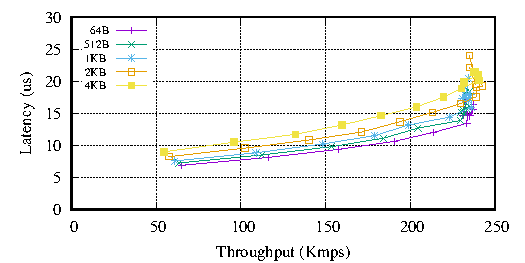
\includegraphics[width=0.97\columnwidth]{figures/benchmark/graphs/figure-performance-vs-size-single-group-up-to-4k}
  \end{subfigure}
  \begin{subfigure}{\columnwidth}
    \advance\leftskip+0.07cm
    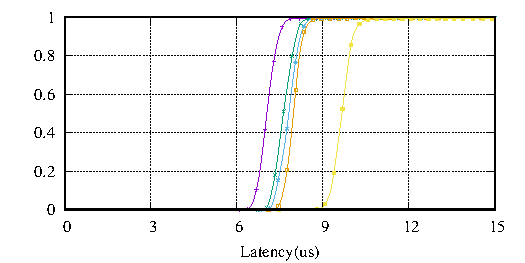
\includegraphics[width=0.96\columnwidth]{figures/benchmark/graphs/figure-performance-vs-size-single-group-cdf-up-to-4k}
  \end{subfigure}
  \begin{subfigure}{\columnwidth}
    \advance\leftskip-0.1cm
    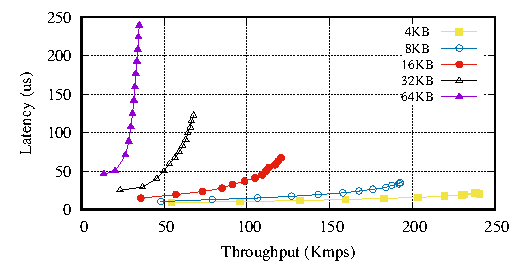
\includegraphics[width=0.99\columnwidth]{figures/benchmark/graphs/figure-performance-vs-size-single-group-from-4k}
  \end{subfigure}
  \begin{subfigure}{\columnwidth}
    \advance\leftskip+0.1cm
    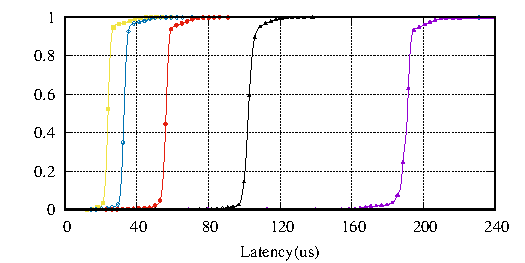
\includegraphics[width=0.96\columnwidth]{figures/benchmark/graphs/figure-performance-vs-size-single-group-cdf-from-4k}
  \end{subfigure}
  \caption{\libname performance with different message sizes: 64B to 2 KB (top) and 4 KB to 32 KB (bottom), throughput versus latency (left) and latency cumulative distribution function for a single client (right).}
  \label{fig:1group_message_size}
\end{figure*}

\subsection{The impact of message size}
\label{sec:evaluation:micro}

In this experiment, conducted on XL170 nodes, we measure \libname throughput and latency for different message sizes.
For each message size, we increase the number of clients until the system is saturated, i.e., throughput stops improving while latency raises.
Figure~\ref{fig:1group_message_size} (left) shows that up to 4KB messages, the impact of message size on the system throughput is negligible, with nearly 250 thousand messages delivered per second. 
As the message size increases past 4KB, the maximum throughput decreases with 35 thousand messages per second for 64KB messages.
The latency cumulative distribution function (CDF) in Figure~\ref{fig:1group_message_size} (right) exhibits minimum latency variation for messages with up to 2KB, around 8 microseconds at $95^{th}$ percentile. At 4KB messages, the latency slightly go up to around 10 microseconds.


\subsection{The performance of atomic multicast}
\label{sec:evaluation:multicast}

The last set of experiments assess \libname behavior in scenarios with up to 8 groups of 3 replicas each, deployed on XL170 machines.
The first experiment comprises executions in which clients send single-group 64-byte messages in setups with 1, 2, 4, and 8 groups.
Figure~\ref{fig:multicast-single-multi-group} (top left) shows the aggregated throughput results when the system is saturated. 
\libname outperforms WBCast by a factor of 3.6$\times$ in all configurations.
These results highlight the benefit of genuine atomic multicast algorithms and show that the throughput grows linearly with the number of groups for single-group messages. 
Since groups do not exchange any information when dealing with single-group messages, the latency CDF is the same for a single client, no matter the number of groups in the system, as depicted in Figure~\ref{fig:multicast-single-multi-group} (middle and bottom left).

%\begin{figure}[htp!]
%  \begin{subfigure}{\columnwidth}
%    \advance\leftskip-0.25cm
%    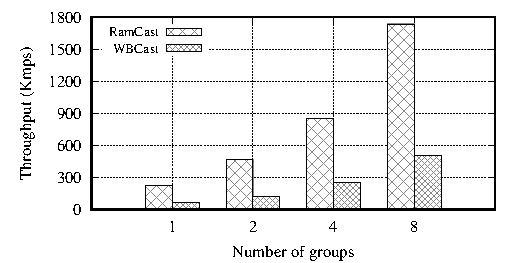
\includegraphics[width=1.01\columnwidth]{figures/benchmark/graphs/figure-genuine-compare-throughput}
%  \end{subfigure}
%  \begin{subfigure}{\columnwidth}
%    \centering
%    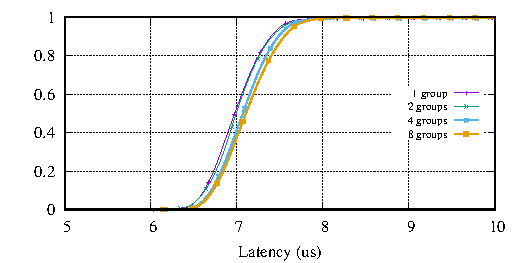
\includegraphics[width=0.95\columnwidth]{figures/benchmark/graphs/figure-genuine-compare-latency-cdf}
%  \end{subfigure}
%  \caption{Performance of atomic multicast when messages are multicast to a single group: throughput (top) and latency cumulative distribution function of a \libname's single client (bottom).}
%  \label{fig:multicast-single-group}
%\end{figure}

The next experiment evaluates the protocols with multi-group messages of 64 bytes addressed to all the groups.
\libname's maximum throughput is greater than WBCast's in every configuration with 233, 145, 80, and 40 thousand messages per second for 1, 2, 4, and 8 destination groups against 63, 50, 35, and 27 thousand for WBCast, as shown in Figure~\ref{fig:multicast-single-multi-group} (top right).
The values correspond to improvements of 3.7$\times$, 2.9$\times$, 2.3$\times$ and 1.5$\times$, respectively.
The difference is even more expressive if we consider the latency for a single client, i.e., when both protocols are contention-free. Figure~\ref{fig:multicast-single-multi-group} (middle right) shows that the latency CDF for \libname with values of 8, 46, 78 and 150~microseconds for 1, 2, 4, and 8 destination groups if we consider the $95^{th}$ percentile. 
The equivalent values for WBCast, as depicted in Figure~\ref{fig:multicast-single-multi-group} (bottom right), are 214, 445, 673, and 1055~microseconds, representing 20$\times$ to 7$\times$ slower delivery times when compared to \libname's.

%\begin{figure}[htp!]
%  \begin{subfigure}{\columnwidth}
%    \advance\leftskip-0.1cm
%    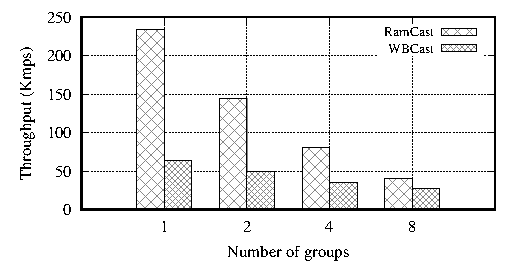
\includegraphics[width=0.99\columnwidth]{figures/benchmark/graphs/figure-multi-dest-compare-throughput}
%  \end{subfigure}
%  \begin{subfigure}{\columnwidth}
%    \centering
%    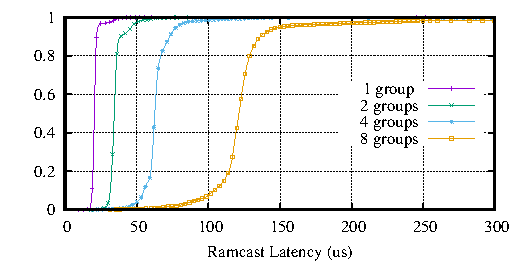
\includegraphics[width=0.95\columnwidth]{figures/benchmark/graphs/figure-multi-dest-compare-latency-cdf-ramcast}
%  \end{subfigure}
%  \begin{subfigure}{\columnwidth}
%    \centering
%    \includegraphics[width=0.95\columnwidth]{figures/benchmark/graphs/figure-multi-dest-compare-latency-cdf-WBCast}
%  \end{subfigure}
%  \caption{Performance comparison of \libname and WBCast for multi-group messages: throughput (top) and latency cumulative distribution function of \libname's (middle) and WBCast's single client (bottom).}
%  \label{fig:multicast-multi-group}
%\end{figure}

\begin{figure*}[ht]
  \begin{subfigure}{\columnwidth}
    \advance\leftskip-0.25cm
    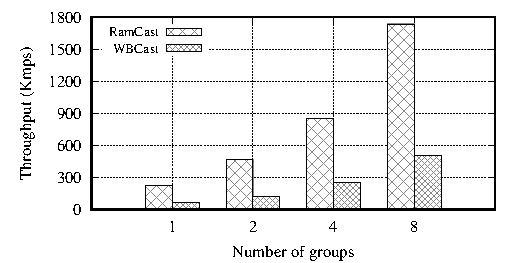
\includegraphics[width=1.01\columnwidth]{figures/benchmark/graphs/figure-genuine-compare-throughput}
  \end{subfigure}
  \begin{subfigure}{\columnwidth}
    \advance\leftskip-0.1cm
    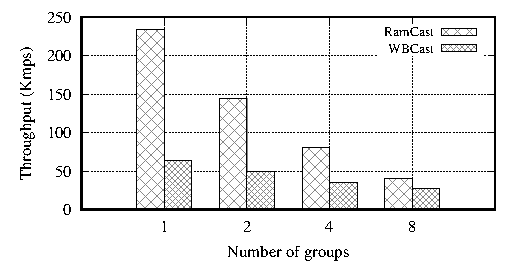
\includegraphics[width=0.99\columnwidth]{figures/benchmark/graphs/figure-multi-dest-compare-throughput}
  \end{subfigure}

  \begin{subfigure}{\columnwidth}
    \centering
    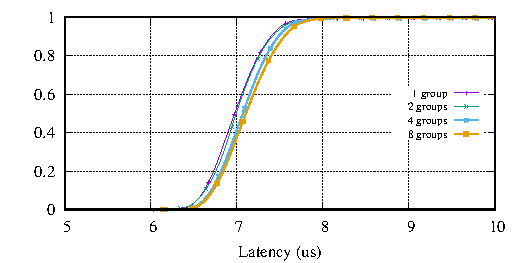
\includegraphics[width=0.95\columnwidth]{figures/benchmark/graphs/figure-genuine-compare-latency-cdf}
  \end{subfigure}
  \begin{subfigure}{\columnwidth}
    \centering
    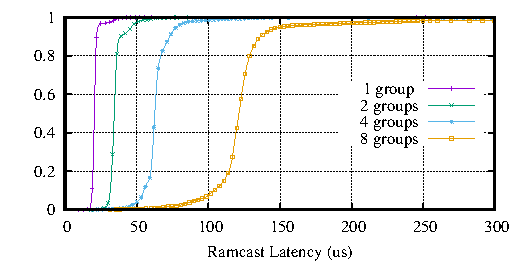
\includegraphics[width=0.95\columnwidth]{figures/benchmark/graphs/figure-multi-dest-compare-latency-cdf-ramcast}
  \end{subfigure}

  \begin{subfigure}{\columnwidth}
    \centering
    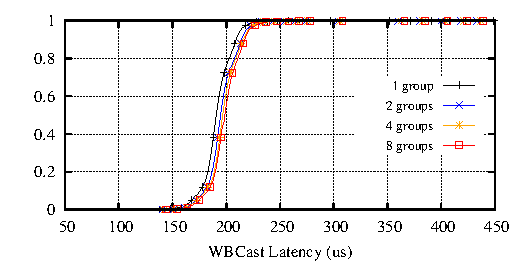
\includegraphics[width=0.95\columnwidth]{figures/benchmark/graphs/figure-genuine-compare-latency-cdf-wbcast}
  \end{subfigure}
  \begin{subfigure}{\columnwidth}
    \centering
    \includegraphics[width=0.95\columnwidth]{figures/benchmark/graphs/figure-multi-dest-compare-latency-cdf-WBCast}
  \end{subfigure}
  \caption{Performance of atomic multicast when messages are multicast to a single group (graphs on the left) and to all groups (graphs on the right). In each case, we show: throughput (top) and latency cumulative distribution function with one client of \libname (middle) and WBCast (bottom).}
  \label{fig:multicast-single-multi-group}
\end{figure*}

\begin{figure}[htp!]
  \begin{subfigure}{\columnwidth}
    \advance\leftskip-0.0cm
    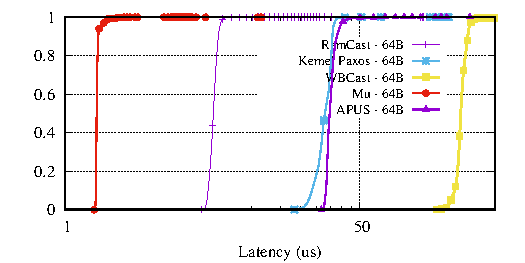
\includegraphics[width=1\columnwidth]{figures/benchmark/graphs/figure-compare-single-group-latency-cdf-64b}
  \end{subfigure}
  \begin{subfigure}{\columnwidth}
    \centering
    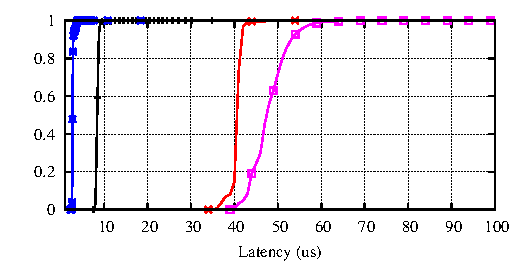
\includegraphics[width=1\columnwidth]{figures/benchmark/graphs/figure-compare-single-group-latency-cdf-1k}
  \end{subfigure}
  \caption{Latency cumulative distribution function for \libname and atomic broadcast protocols with a single client: 64-byte messages (top) and 1K-byte messages (bottom).}
  \label{fig:broadcast}
\end{figure}



\subsection{\libname's inherent performance}
\label{sec:evaluation:broadcast}

This experiment assesses how each protocol behaves in a scenario with a single group of three replicas, and 64-byte and 1-kilobyte messages.
Figure~\ref{fig:broadcast} (top) shows that, for 64-byte messages, \libname outperforms the competitors with approximately 200 thousand messages per second. 
Kernel Paxos comes close with 170 thousand messages per second, while WBCast saturates sooner, with less than 60 thousand messages per second.
For larger messages, \libname kept the same performance, while the other protocols had the throughput reduced by half.
Figure~\ref{fig:broadcast} (bottom) confirms the superior results for \libname. The median latency for WBCast with small messages and a single client is twenty times greater than the same measurement for \libname.



%!TEX root =  main.tex
\section{Related work}
\label{sec:related-work}

\libname is at the intersection of atomic multicast protocols (\S\ref{sec:rwamcast}), 
RDMA-based systems (\S\ref{sec:rwrdmasys}), and RDMA-based consensus protocols (\S\ref{sec:rwrdmacons}).


\subsection{Atomic multicast}
\label{sec:rwamcast}

Atomic multicast is a well-studied problem. Skeen's algorithm (described in \S\ref{sec:bblocks}) is possibly the first atomic multicast algorithm.
%Processes in Skeen assign timestamps to messages ensure that destinations agree
%on the final timestamp assigned to each message, and deliver messages following
%this timestamp order. The precise way in which these properties are ensured
%varies from one algorithm to another. 
Even though it is not fault-tolerant, it
is genuine: processes only communicate if they are in the destinations of the messages. 
Later timestamp-based genuine atomic multicast algorithms 
implemented fault-tolerant versions of Skeen's protocol. 
FastCast \cite{Coelho2017} speeds up the delivery of messages by overleaping some parts of the protocol (i.e., the order proposed by the leader and the consensus needed to decide on the proposed order).
In good runs, FastCast delivers multi-group messages in 4 communication steps.
White-Box Atomic Multicast \cite{gotsman2019white} further improves 
latency with a protocol that combines Paxos and a fault-tolerant version of Skeen's protocol.
White-Box Atomic Multicast delivers multi-group messages in 3 communication steps at the leaders of the involved groups and 4 communication steps at the followers.
\libname improves on White-Box Atomic Multicast in that both leaders and followers can deliver a multi-group message in 3 communication steps.

Ring-based protocols \cite{delporte2000fault, bezerra2015ridge,
marandi2012multi} proposed a different approach to high throughput by
propagating messages along a predefined ring overlay and ensuring atomic multicast
properties by relying on this topology. However, ring-based algorithms are
non-genuine: involved processes communicate with processes outside the
destination groups to deliver messages. The time complexity of these algorithms is
proportional to the number of destination groups.

\subsection{RDMA systems}
\label{sec:rwrdmasys}

Remote Direct Memory Access (RDMA) \cite{kalia2016design} is an interface that
allows servers to read and write the memory of a remote server directly. Over
the years, RDMA has become an active area of research for its high throughput,
low latency, and low CPU overhead. RDMA techniques have been implemented in
various architectures, including Infiniband \cite{pfister2001introduction}, RoCE
\cite{beck2011performance}, and iWRAP \cite{rashti200710}. RDMA has already been
explored and applied in a variety of applications, from key/value stores
\cite{FaRM, kalia2014using, mitchell2013using, wei2015fast}, to databases
\cite{binnig2015end, huang2019rdma}, and distributed file systems
\cite{islam2012high, li2009early, wu2003pvfs}. Pilaf \cite{mitchell2013using} is
a distributed in-memory key-value store that implements client-lookup operations
with one-sided RDMA reads. In contrast, in HERD \cite{kalia2014using}, clients use
one-sided RDMA writes to send requests to servers which poll their receive RDMA
buffers to process requests. FaRM \cite{FaRM} proposes a distributed computing
platform, which provides the transactional interface for applications to access
the shared memory. NVFS \cite{islam2012high} provides a novel design of HDFS
with byte-addressable NVM and RDMA network. Octopus \cite{lu2017octopus} is a
distributed, shared persistent memory file system that combines RDMA and NVM's
new features by redesigning the software. Besides, many optimization guidelines
was proposed by Kalia et al. \cite{kalia2016design} to enhance performance of
RDMA system. 
We have applied many of the mentioned best practices
in the implementation of \libname.


\subsection{RDMA-based consensus}
\label{sec:rwrdmacons}

RDMA has received limited attention in the context of consensus
protocols, and only a few crash-tolerant replication protocols based on RDMA 
have been proposed. DARE \cite{DARE} aims to optimize for low latency in replica
communication. The consensus leader in DARE replicates requests to its follower
with RDMA one-sided read/write operations, and makes use of permissions when
changing leaders. APUS \cite{APUS} improves upon DARE. APUS
combines RDMA with Paxos and focuses on scalability with the number of
connections and replicas. APUS is based on intercepting inbound socket calls, so
it does not require modifying applications for integration. Derecho
\cite{jha2019derecho} provides an RDMA-enabled state machine replication while
structuring applications into groups, subgroups, and shards. Derecho only needs
a leader for group reconfiguration. 
Mu \cite{Mu} exploits Protected Memory Paxos and colocates the client with the leader of Paxos to reach low latency.
Similarly to Mu, \libname also relies on RDMA's protected memory to order single-group messages efficiently.
However, \libname cannot colocate clients and leaders since it implements atomic multicast.
This happens because clients may multicast a message to different groups and colocating all leaders in the same host defeats the purpose of atomic multicast.

%However, these protocols focus on building consensus on top of RDMA primitives.
%To our knowledge, there is no previous work that solved atomic multicast with
%RDMA.


% \section{State machine replication}

% State machine replication (SMR) was first introduced by Lamport in \cite{Lam78}. Schneider \cite{Sch90} then presented a more systematic
% approach to the design and implementation of SMR protocols. Since then, SMR has
% become a well-known approach to replication and has been extensively studied,
% both in academia (e.g., \cite{Kapritsos:2012um, Kotla:2004ep, santos2013htsmr,
% Mencius}) and in the industry (e.g., \cite{corbett2013spanner}). SMR provides strong consistency guarantees, which
% come from total order and deterministic execution of commands. Traditional SMR
% relies on a consensus protocol to define a common order among replicas for the execution of 
% commands. Deterministic execution is usually ensured by having every replica
% execute the set of ordered commands sequentially.

% % 

\section{Conclusion}
\label{sec:conclusion}

Atomic multicast is a fundamental communication abstraction in the design of scalable and highly available strongly consistent distributed systems.
This paper presents \libname, the first genuine atomic multicast protocol tailor-made for the shared-memory model.
In addition to introducing a novel algorithm that leverages the permission mechanism of RDMA's write operations to reduce the number of communication steps, we also have implemented and evaluated the protocol under a large range of parameters.
The results show that \libname outperforms both a kernel-space atomic broadcast and a recent state-of-the-art message-passing genuine atomic multicast algorithm.




%!TEX root =  main.tex

\newcommand{\Pend}{\ensuremath{\mathit{ToOrder}}\xspace}
\newcommand{\Done}{\ensuremath{\mathit{Ordered}}\xspace}
\newcommand{\Decided}{\ensuremath{\mathit{Decided}}\xspace}
\newcommand{\Buffer}{\ensuremath{\mathcal{B}}\xspace}

\clearpage
\section{Proof of correctness}

\begin{proposition}
\textit{(Uniform integrity)~For any message $m$, every process $p$ delivers $m$ at most once, and only if $p$ is a destination of $m$ and $m$ was previously multicast.}
\end{proposition}
\vspace{2mm}
\noindent
{\sc Proof:} 
Process $p$ delivers $m$ at Task 6 if $m$'s state is \ordered. 
After delivering $m$, $p$ sets $m$'s state to \done, and thus $m$ cannot be delivered more than once.

Let $c$ be the client that multicasts $m$ to groups in $dst$, and let $p$ be in group $g$. 
From Task 6, $p$ only delivers $m$ if it is in $p$'s $M$ buffer and $m$'s state is \ordered. 
Message $m$'s state is set to \ordered\ in Task 5 if its current state is \mcast.
A message's state is set to \mcast\ in procedure $Relay$, which is invoked in two cases:
(a)~by client $c$ upon multicasting $m$ (Task 1) to groups in $dst$, in which case $g \in dst$; or 
(b)~by some process $q$ that suspects $c$ (Task 10), has $m$ in its buffer in state \mcast, and $g$ is a destination of $m$.
In case (b), $m$ was written in $q$'s buffer either (b.1) directly by $c$ or (b.2) indirectly by some other process.
In any case, there is some process $r$ such that $m$ is included in $r$'s buffer by $c$.
It follows from Task 1 that $p$ is a destination of $m$ and $m$ was multicast by client $c$.\hfill$\Box$

%\begin{lemma}
%If a correct process $p$ in $g$ includes tuple $T$ in \Pend, then eventually processes in $g$ decide on a sequence of tuples that contains $T$.
%\label{lemma:Y}
%\end{lemma}
%\noindent
%{\sc Proof:} 
%Process $p$ includes $T$ in \Pend either in Task 1 or in Task 2.
%In both cases, $T$ was r-delivered by $p$ and from the properties of reliable broadcast, every correct process in $g$ will r-deliver $T$ and include it in \Pend.
%Let $t$ be a time after which all faulty processes have failed.
%Thus, after $t$ there is a time when all \Pend sequences from processes that propose in consensus contain $T$.
%By the uniform integrity property of consensus, $T$ is eventually included in a decision of consensus.\hfill$\Box$
%
%
%\begin{lemma}
%For each correct process $p$ that has tuple $(\textsc{sync-hard}, h, x, m)$ in \Buffer, $p$ eventually replaces the entry by $(\textsc{final}, \bot, ts, m)$ in \Buffer where $ts$ is the maximum timestamp $x$ in the \textsc{sync-hard} tuples that concern $m$.
%\label{lemma:X}
%\end{lemma}
%\noindent
%{\sc Proof:} 
%To include $(\textsc{sync-hard}, h, x, m)$ in \Buffer, $p$ has decided on a sequence that contains either \\
%(a)~a $(\textsc{set-hard}, h, x, m)$ tuple if $m$ is local, or 
%(b)~a $(\textsc{sync-hard}, h, x, m)$ tuple if $m$ is global.
%In case (a), $(\textsc{sync-hard}, h, x, m)$ will be trivially replaced by $(\textsc{final}, \bot, x, m)$ in Task 5.
%In case (b), some process proposed a $\Pend \setminus \Done$ sequence that contains $(\textsc{sync-hard}, h, x, m)$.
%The \textsc{sync-hard} tuple is included in \Pend in Task 2 upon r-delivering tuple $(\textsc{send-hard}, h, x, m)$, which was r-multicast in Task 4, upon the decision of a sequence with $(\textsc{set-hard}, h, x, m)$.
%Thus, $(\textsc{set-hard}, h, x, m)$ was included in \Pend at Task 1, as a result of the r-delivery of $(\textsc{start}, \bot, \bot, m)$, which is r-multicast to all of $m$'s destinations.
%Every group $h$ in $m.dst$ upon r-delivering $(\textsc{start}, \bot, \bot, m)$ adds tuple $(\textsc{set-hard}, h, x, m)$ to \Pend, which from Lemma~\ref{lemma:Y} is eventually included in a consensus decision and results in the r-multicast of $(\textsc{send-hard}, h, x, m)$ to members of $m.dst$.
%When a process r-delivers $(\textsc{send-hard}, h, x, m)$, it adds $(\textsc{sync-hard}, h, x, m)$ to \Pend and, from Lemma~\ref{lemma:Y}, the tuple is decided in an instance of consensus, leading to the inclusion of $(\textsc{sync-hard}, h, x, m)$ in \Buffer.
%Once there is a tuple $(\textsc{sync-hard}, h, x, m)$ in \Buffer for each group $h$ in $m.dst$, $p$ replaces the \textsc{sync-hard} tuples by $(\textsc{final}, \bot, ts, m)$.\hfill$\Box$
%
%\begin{lemma}
%If a correct process $p$ includes $(\textsc{final}, \bot, ts, m)$ in \Buffer, then $p$ eventually a-delivers $m$.
%\label{lemma:Z}
%\end{lemma}
%\noindent
%{\sc Proof sketch:} 
%Assume for a contradiction that $q$ does not a-deliver $m$.
%Thus, there is some tuple $(z,h,y,m')$ in \Buffer such that $m \neq m'$ and $y < ts $.
%We first show that eventually any entry $(z,h,y,m')$ added in \Buffer after $(\textsc{final}, \bot, ts, m)$ is in \Buffer has a timestamp bigger than $ts$.
%Message $m$ only has a \textsc{final} tuple in \Buffer after it received \textsc{sync-hard} tuples from all of $m$'s destinations.
%When $q$ includes $(\textsc{sync-hard}, h, x, m)$ in \Buffer in Task 4, $q$ updates $C_h$ such that it contains the maximum between it current value and $x$.
%Since the next \textsc{set-hard} event that $q$ handles for a message $m''$ will increment $C_h$, it follows that $m''$ will have a timestamp bigger than $ts$.
%
%We now show that every message that contains a timestamp smaller than $m$'s final timestamp $ts$ is eventually a-delivered and removed from \Buffer.
%Let $(z,h,y,m')$ be an entry in \Buffer such that $y<ts$.
%Either $z$ is \textsc{final} or it is \textsc{sync-hard} and from Lemma~\ref{lemma:X} $z$ the tuple will eventually be replaced by a \textsc{final} tuple.
%Thus, from Task 5 message $m'$ will be eventually a-delivered and removed from \Buffer, a contradiction.
%We conclude then that $q$ eventually a-delivers $m$.\hfill$\Box$

\vspace{2mm}
\begin{lemma}
If all correct processes in the destination of an atomically multicast message $m$ have $m$ in their $M$ buffer in the \mcast\ state, then they eventually set $m$ to the \ordered\ state.
\label{lemma:X}
\end{lemma}
\vspace{2mm}
\noindent
{\sc Proof:} 
Let $m$ be addressed to groups in $dst$ and $q$ be a correct process addressed by $m$.
We claim that for each $h \in dst$, $q $ will have a timestamp for $h$ that is acknowledged by a quorum of processes in $h$.
By the leader election oracle and the fact that each group has a majority of correct processes, group $h$ eventually has a stable correct leader $l$.
Either (a) $l$ executes Task 2 and proposes its clock value as $h$'s timestamp or (b) $l$ executes Task 7 to replace a suspected leader.
In (b), $l$ sends a \textsc{catch\_up} message to all processes and will receive for each group $g \in dst$ the timestamp proposed in $g$, if any, and the corresponding acknowledgements from processes in $g$ (Task 8).
For the case where $h=g$, $l$ will pick the timestamp decided by a previous leader or choose one if no timestamp has been decided (Task 9).
Thus, in both cases (a) and (b), the leader writes the chosen timestamp in the $M$ buffer of each process in $h$ and in the leaders of other groups in $dst$.
From Task 3, every follower in $h$ will acknowledge this timestamp in the buffer of each process in the destination of $m$.
From Task 4, when $l$ has a timestamp from $g \neq h$, $l$ writes the timestamp in the buffer of its followers, which concludes the claim.
Therefore, eventually $q$ has a timestamp for every group in $dst$, can compute $m$'s final timestamp, and set $m$'s state as \ordered.

\pagebreak
\begin{lemma}
If a correct process $p$ has an atomically multicast message $m$ in its $M$ buffer in the \ordered\ state, then $p$ eventually delivers $m$.
\label{lemma:Z}
\end{lemma}
\vspace{2mm}
\noindent
{\sc Proof:} 
Assume for a contradiction that $q$ does not deliver $m$.
Thus, there is some message $m'$ in the buffer such that $m \neq m'$, $m'$'s timestamp is smaller than $m$'s timestamp, and $m'$'s state is not \done.

We first show that any message added in the buffer after $m$ becomes \ordered\ has a timestamp bigger than $m$'s timestamp.
Message $m$ only becomes ordered after it has timestamps from all groups in $m$'s destinations $dst$.
When $q$ reads a timestamp $x$ for $m$ from some group in $dst$, $q$ updates its clock such that it contains the maximum between its current value and $x$.
Since the next event that $q$ handles for a message $m''$ will increment its clock, it follows that $m''$ will have a timestamp bigger than $x$.

We now show that every message that contains a timestamp smaller than $m$'s final timestamp $ts$ is eventually delivered and its state set to \done.
To see why, let $m'$ be the message with the smallest timestamp in the buffer.
Thus, such a message is eventually delivered and its state set to \ordered.
Eventually, $m$ will be the message in the buffer with smallest timestamp and therefore delivered, a contradiction.
We conclude then that $q$ eventually delivers $m$.\hfill$\Box$


\vspace{2mm}
\setcounter{proposition}{1}
\begin{proposition}
\textit{(Validity)~If a correct client $c$ multicasts a message $m$, then eventually every correct process $p$ in $m$'s destination $dst$ delivers $m$.}
\end{proposition}
\vspace{2mm}
\noindent
{\sc Proof:} 
Upon multicasting $m$, $c$ relays $m$ to groups in $dst$ (see Task 1).
The Relay procedure then copies $m$ to the $M$ buffer of every correct process $p$ in groups in $dst$ and sets its state to \mcast.
From Lemma~\ref{lemma:X}, it follows that every correct process $p$ set $m$'s state to \ordered.
From Lemma~\ref{lemma:Z}, $p$ eventually delivers $m$.\hfill$\Box$

\vspace{2mm}
\begin{proposition}
  \textit{(Uniform agreement)~If a process $p$ delivers a message $m$, then eventually all correct processes $q$ in $m$'s destination $dst$ deliver $m$.}
\end{proposition}
\vspace{2mm}
\noindent
{\sc Proof:} 
For process $p$ to deliver $m$, from Task 6, $p$ has a timestamp for every group $h$ in $dst$ in the $M$ buffer such that $ts$ is the largest among these timestamps.
Moreover, there is no message $m'$ in the buffer such that $m \neq m'$, $ts < y$, where $y$ is a timestamp assigned to $m'$, and $m'$ is not ordered.

We first show by contradiction that $q$ eventually has $m$ in its $M$ buffer.
Let $c$ be the client that multicasts $m$.
If $c$ is correct then, $c$ writes $m$ in $q$'s buffer, so consider that $c$ fails before it can write $m$ in $q$'s buffer.
Since $p$ delivers $m$, it has a quorum of acknowledges from each group in $dst$.
Any quorum includes at least one correct process, which from Task 10, eventually suspects $c$ and relays $m$ to all processes in $dst$, including $q$, a contradiction.

It follows from Lemma~\ref{lemma:X} that $q$ eventually sets the state of $m$ to \ordered\ in its buffer, and 
from Lemma~\ref{lemma:Z} that $q$ eventually delivers $m$.\hfill$\Box$

\vspace{2mm}
\begin{proposition}
  \textit{(Uniform prefix order)~For any two messages $m$ and $m'$ and any two processes $p$ and $q$ such that $\lbrace p, q\rbrace \subseteq \mathit{dst} \cap \mathit{dst'}$, where $dst$ and $dst'$ are the groups addressed by $m$ and $m'$, respectively, if $p$ delivers $m$ and $q$ delivers $m'$, then either $p$ delivers $m'$ before $m$ or $q$ delivers $m$ before $m'$.}
\end{proposition}
\vspace{2mm}
\noindent
{\sc Proof:} 
The proposition trivially holds if $p$ and $q$ are in the same group, so assume $p$ is in group $g$ and $q$ is in group $h$ and suppose, by way of contradiction, that $p$ does not deliver $m'$ before $m$ nor does $q$ deliver $m$ before $m'$. 
Without loss of generality, suppose that $m$'s timestamp $ts$ is smaller than $m'$'s timestamp $ts'$. 

We claim that $q$ inserts $m$ into the $M$ buffer before delivering $m'$. 
In order for $m$ (respectively, $m'$) to be delivered by $p$ (resp., $q$), $p$'s (resp., $q$'s) $M$ buffer must contain a timestamp $ts_g$ from group $g$ and $ts_h$ from group $h$ (resp., $ts_g'$ from group $g$ and $ts_h'$ from group $h$).

From Task 2 (or Task 9 if some process has suspected the leader), the leader $l$ in group $g$ must have included the timestamp $ts_g$ for message $m$ and $ts_g'$ for message $m'$ in $p$'s $M$ buffer and both timestamps have been acknowledged by a quorum of processes in group $g$.
Assume that the leader $l$ has written $ts_g$ before $ts_g'$ to the $M$ buffer of every follower in group $g$ and the leader $l_h$ in group $h$. 
From Task 2, we have $ts_g < ts_g'$.
Therefore, from Task 4, $l_h$ will write to the $M$ buffer of every follower in group $h$, including $q$, both $ts_g$ for message $m$ and $ts_g'$ for message $m'$.

%From Task 4, for $p$ to include a \textsc{sync-hard} tuple in \Buffer, $p$ must have decided a sequence that contains $(\textsc{sync-hard}, g, x, m)$ (recall that $m$ is a global message).
%Thus, some process in $g$ included $(\textsc{sync-hard}, g, x, m)$ in \Pend, after r-delivering tuple  $(\textsc{send-hard}, g, x, m)$.
%With a similar argument, some process in $g$ included $(\textsc{sync-hard}, g, x', m')$ in \Pend, after r-delivering tuple $(\textsc{send-hard}, g, x', m')$.
%Let $r$ and $s$ be the processes that r-multicast messages $(\textsc{send-hard}, g, x, m)$ and $(\textsc{send-hard}, g, x', m')$, respectively, at Task 4.
%Therefore, $r$ and $s$ decided sequences that include the \textsc{set-hard} tuples.
%Assume that $(\textsc{set-hard}, g, x, m)$ is decided before $(\textsc{set-hard}, g, x', m')$.
%Therefore, before r-multicasting $(\textsc{send-hard}, g, x', m')$, $s$ r-multicast $(\textsc{send-hard}, g, x, m)$.
%From the FIFO properties of reliable multicast, $q$ r-delivered the tuples in the order above and we can show that $(\textsc{sync-hard}, g, x, m)$ appears in \Buffer before $(\textsc{set-hard}, g, x', m')$, which proves our claim.

Consequently, from the claim, $q$ delivers $m$ before $m'$ since $m.ts < m'.ts$, a contradiction that concludes the proof.
\hfill$\Box$

\vspace{2mm}
\begin{proposition}
\textit{(Uniform acyclic order)~Let relation $<$ be defined such that $m < m'$ iff there exists a process that delivers $m$ before $m'$.  The relation $<$ is acyclic.}
\end{proposition}
\vspace{2mm}
\noindent
{\sc Proof:} 
Suppose, by way of contradiction, that there exist messages $m_1, ..., m_k$ such that $m_1 < m_2 < ... < m_k < m_1$. 
From Task 6, processes deliver messages following the order of their final timestamps.
Thus, there must be processes $p$ and $q$ such that the final timestamps they assign to $m_1$, $ts_p$ and  $ts_q$, satisfy $ts_p < ts_q$, a contradiction since both $p$ and $q$ have the same timestamps for each group in $dst$ in Task 6.
\hfill$\Box$

\vspace{2mm}
\begin{theorem}
RamCast implements atomic multicast.
\end{theorem}
\vspace{2mm}
\noindent
{\sc Proof:} 
This follows directly from Propositions 1 through 5.\hfill$\Box$



%\pagebreak
\bibliographystyle{ieeetr}
\bibliography{references}
\newpage

\end{document}
